\documentclass[11pt]{article}
\usepackage[margin=1in]{geometry}
\usepackage{graphicx}
\usepackage{float}
\usepackage{booktabs}
\usepackage{amsmath}

\graphicspath{{../results/}}

\title{CS683 Programming Assignment II\\Data Prefetching and Cache Replacement}
\date{}

\begin{document}
\sloppy
\maketitle

\section*{Summary of results}
\begin{table}[H]
\centering
\small
\setlength{\tabcolsep}{4pt}
\begin{tabular}{lp{0.28\linewidth}rrr}
\toprule
Task & Mechanism (baseline) & Avg.\ speedup & Best trace & Key metric\\
\midrule
1B & SPP at L1D (no PF) & 1.0024 & Trace1: 1.0042 & accuracy 50.5\% (IP-stride 35.7\%)\\
2A & I-RRIP at L2 (LRU) & 1.0079 & Trace2: 1.0241 & Trace2 L2 instr.\ MPKI $-35.3\%$\\
2B & Dynamic I-RRIP at L2 (LRU) & 1.0068 & Trace2: 1.0223 & Trace2 L2 instr.\ MPKI $-33.0\%$\\
3 & SPP + PF-aware Dyn-I-RRIP (no PF) & 1.0069 & Trace2: 1.0163 & avg.\ IPC 0.2903\\
\bottomrule
\end{tabular}
\caption{Headline results (baseline in parentheses; PF = L1D prefetching).
Average speedups are geometric means over the three traces.}
\label{tab:summary}
\end{table}

\begin{itemize}
  \item \textbf{Task 1 (prefetching):} SPP combines a uniform-stride predictor
        with a signature-based pattern table and accuracy-based throttling. It
        is more accurate than IP-stride on every trace and has the lowest L1D
        load MPKI, but both prefetchers give speedups below 0.6\% because at
        most 5.8\% of the L1D load misses are predictable from per-IP strides.
        Storage: about 6.7\,KB.
  \item \textbf{Task 2A (I-RRIP):} protecting instruction lines at insertion,
        promotion and eviction cuts L2 instruction misses on every trace and
        gives 2.4\% speedup on the code-heavy Trace2. Storage: 3\,KB.
  \item \textbf{Task 2B (Dynamic I-RRIP):} set dueling with 32 SRRIP leader sets
        keeps about 87\% of the I-RRIP gain while being able to fall back to
        SRRIP. The result is insensitive to the threshold and the number of
        leaders. Storage: 3\,KB + 60 bits.
  \item \textbf{Task 3 (SPP + prefetch-aware Dynamic I-RRIP):} prefetched
        lines are inserted into the L2 at RRPV 3, prefetch hits are not
        promoted and prefetches are not counted by the leader sets. The
        combination keeps SPP's L1D gains and most of Dynamic I-RRIP's L2
        instruction-miss reduction, and has the highest average IPC, but its
        speedup only matches Dynamic I-RRIP's and it does not beat both
        standalone mechanisms on every trace. No extra storage.
\end{itemize}

\section*{Experimental setup}
All runs use the ChampSim build from the PA2 repository with 25M warmup and 25M
simulated instructions on the three provided traces (Trace1-003, Trace2-001,
Trace3-002). Each experiment changes only the mechanism under study:
\begin{itemize}
  \item \textbf{Task 1}: only the L1D prefetcher changes; every cache uses LRU
        and all other prefetchers are off. Baseline: no L1D prefetching.
  \item \textbf{Task 2}: only the L2 replacement policy changes; all
        prefetchers are off and every other cache uses LRU. Baseline: LRU at the
        L2 (1024 sets $\times$ 8 ways, 512\,KB).
  \item \textbf{Task 3}: SPP at the L1D together with prefetch-aware Dynamic
        I-RRIP at the L2; every other cache uses LRU. Baseline: no L1D
        prefetching with LRU at the L2 (the Task 1B baseline).
\end{itemize}
Metrics:
\begin{itemize}
  \item \textbf{Speedup} $= \text{IPC with the mechanism} / \text{IPC of the baseline}$
        on the same trace. The ``Average'' speedup is the geometric mean over
        the three traces; every other average is the arithmetic mean.
  \item \textbf{MPKI}: misses per 1000 instructions, from the ChampSim
        statistics (\texttt{L1D LOAD} line for Task 1; \texttt{L2C LOAD},
        \texttt{L2C INSTRUCTION LOAD} and \texttt{L2C DATA LOAD} lines for
        Task 2).
  \item \textbf{Prefetch accuracy}: the \texttt{ACCURACY} field of the
        \texttt{L1D USEFUL LOAD PREFETCHES} line
        (useful load prefetches / prefetches issued to the lower level).
  \item \textbf{Prefetch coverage}
        $= \dfrac{\text{L1D load misses (baseline)} - \text{L1D load misses (prefetcher)}}
                 {\text{L1D load misses (baseline)}}$.
\end{itemize}
The raw outputs are in \texttt{results/task1b}, \texttt{results/task2a},
\texttt{results/task2b} and \texttt{results/task3}. Task 1 tables and plots were produced by
\texttt{scripts/task1b\_metrics.py}; Task 2 tables and plots by
\texttt{scripts/parse\_results.py}, \texttt{scripts/plot\_results.py} and
\texttt{scripts/plot\_task2b.py}; Task 3 tables and plots by
\texttt{scripts/task3\_metrics.py}.

%======================================================================
\section{Task 1A: IP-stride prefetcher}

\texttt{prefetcher/ip\_stride.l1d\_pref} keeps a 24-entry, fully associative
table of \emph{IP trackers}. Each tracker holds the low 8 bits of the load IP
(\texttt{MASK\_IP = 0xFF}), the last cache-line address that IP touched, the
last stride it saw and an LRU rank.

On every L1D access the prefetcher:
\begin{enumerate}
  \item Looks up the IP. On a miss it replaces the LRU tracker, records the
        current line address with stride 0 and returns without prefetching.
  \item On a hit it computes the stride (in cache lines) from the last address.
        A zero stride is ignored.
  \item If the new stride equals the stored stride (the same stride seen twice
        in a row), it issues prefetches for
        $\text{addr} + k \cdot \text{stride}$, $k = 1 \ldots 3$
        (\texttt{PREFETCH\_DEGREE = 3}). It stops at the first target that
        leaves the 4\,KB page of the demand access. A prefetch fills the L1D
        when fewer than half of the MSHRs are in use and only the L2 otherwise.
  \item It stores the new address and stride and moves the tracker to MRU.
\end{enumerate}

The design has no confidence counter (a single repeat of a stride is enough to
prefetch), a fixed degree and no feedback on whether its prefetches are useful.
It only captures constant strides: a repeating multi-stride sequence such as
$(+1,+2,+2,+2,+3)^n$ almost never shows two equal strides in a row in a way that
predicts the next one. SPP (Task 1B) addresses all three points.

%======================================================================
\section{Task 1B: Stride Pattern Prefetcher (SPP)}

\subsection{Design}
SPP (\texttt{prefetcher/spp.l1d\_pref}) works on cache-line addresses and keeps
one table indexed by the low 8 bits of the IP. Each IP entry contains two
predictors that are trained on every access with a non-zero stride:

\paragraph{Uniform-stride predictor.}
Each IP entry has a \emph{monitored stride} and a 2-bit saturating confidence
counter (0 = no confidence, 2 = high confidence). If the new stride equals the
monitored stride the counter is incremented; otherwise it is decremented, and
once it is already 0 the monitored stride is replaced by the new stride. So a
constant stride needs to repeat twice before it is trusted, and a broken pattern
loses the right to prefetch after a single mismatch.

\paragraph{Non-uniform-stride predictor.}
Each IP entry keeps the history of its last 8 strides
(\texttt{HISTORY\_LEN = 8}). This history is the \emph{signature}. A per-IP
pattern table of up to 24 entries maps a signature to the stride that followed
it, with a 7-bit confidence and an LRU age. On every access the entry for the
\emph{previous} signature is trained with the new stride: a correct prediction
increments its confidence, a wrong prediction halves it, and a wrong prediction
at confidence 0 replaces the predicted stride. The new stride is then shifted
into the history. When the pattern table is full, the entry with the lowest
$\text{confidence} - \text{age}$ is evicted, so stale and unreliable patterns
go first. An 8-stride signature is long enough to tell apart the positions
inside a repeating sequence such as $(+1,+2,+2,+2,+3)^n$, where the
\texttt{+2} stride is followed by different strides depending on where it occurs.

\paragraph{Classification and prefetching.}
The uniform predictor has priority. If the IP's uniform confidence is high (2),
SPP prefetches $\text{line} + k \cdot \text{stride}$ for
$k = 1 \ldots \text{degree}$. Otherwise it falls back to the pattern
predictor: it looks up the current signature, takes the predicted stride, shifts
it into a copy of the signature and repeats the lookup, walking up to
\emph{degree} steps ahead as long as each signature is found. An IP therefore
moves to non-uniform prediction as soon as its constant stride breaks, and back
to uniform prediction once the constant stride has repeated twice.

\paragraph{Page boundary and MSHR.}
No prefetch crosses the 4\,KB page of the demand access: the uniform path stops
at the first out-of-page target, and the pattern path skips out-of-page targets.
Prefetches are only issued while at least 3 MSHR entries are free, so they never
starve demand misses. Strides outside $[-128, 127]$ lines cannot be stored in
8 bits; such an access counts as a uniform-stride mismatch, clears the stride
history and issues no prefetch.

\paragraph{Accuracy-based throttling.}
The prefetch degree is global and starts at 1. Every 256 trained accesses
(\texttt{EPOCH\_LEN}) SPP reads ChampSim's L1D counters for prefetches issued to
the lower level and useful prefetches, and computes the accuracy of the
prefetches issued during that epoch:
\[
  \text{acc} = \frac{\Delta\,\text{useful}}{\Delta\,\text{issued}}, \qquad
  \text{degree} \leftarrow
  \begin{cases}
    \min(\text{degree} + 1,\ 8) & \text{acc} > 0.6\\
    \max(\text{degree} - 1,\ 1) & \text{acc} < 0.3\\
    \text{degree} & \text{otherwise}
  \end{cases}
\]
Epochs in which no prefetch was issued leave the degree unchanged.

\subsection{Results}

\begin{table}[H]
\centering
\begin{tabular}{lrrr rr rrr}
\toprule
& \multicolumn{3}{c}{IPC} & \multicolumn{2}{c}{Speedup} & \multicolumn{3}{c}{L1D load MPKI}\\
\cmidrule(lr){2-4}\cmidrule(lr){5-6}\cmidrule(lr){7-9}
Trace & None & IP-stride & SPP & IP-stride & SPP & None & IP-stride & SPP\\
\midrule
Trace1-003 & 0.2322 & 0.2334 & 0.2332 & 1.0051 & 1.0042 & 10.679 & 10.119 & 10.062\\
Trace2-001 & 0.2511 & 0.2512 & 0.2513 & 1.0002 & 1.0008 & 13.534 & 13.436 & 13.446\\
Trace3-002 & 0.3821 & 0.3830 & 0.3829 & 1.0024 & 1.0023 &  3.403 &  3.318 &  3.285\\
\midrule
Average    & 0.2885 & 0.2892 & 0.2891 & 1.0026 & 1.0024 &  9.205 &  8.957 &  8.931\\
\bottomrule
\end{tabular}
\caption{IPC, speedup over no prefetching and L1D load MPKI.}
\label{tab:t1-perf}
\end{table}

\begin{table}[H]
\centering
\begin{tabular}{l rr rr rr rr}
\toprule
& \multicolumn{2}{c}{Accuracy (\%)} & \multicolumn{2}{c}{Coverage (\%)}
& \multicolumn{2}{c}{Prefetches issued} & \multicolumn{2}{c}{Useful prefetches}\\
\cmidrule(lr){2-3}\cmidrule(lr){4-5}\cmidrule(lr){6-7}\cmidrule(lr){8-9}
Trace & IP-stride & SPP & IP-stride & SPP & IP-stride & SPP & IP-stride & SPP\\
\midrule
Trace1-003 & 52.79 & 60.72 & 5.24 & 5.78 & 30988 & 28454 & 16359 & 17278\\
Trace2-001 & 38.13 & 57.47 & 0.73 & 0.65 & 11472 &  5211 &  4374 &  2995\\
Trace3-002 & 16.09 & 33.36 & 2.51 & 3.48 & 17013 &  9496 &  2738 &  3168\\
\midrule
Average    & 35.67 & 50.52 & 2.83 & 3.30 & & & & \\
\bottomrule
\end{tabular}
\caption{L1D prefetch accuracy, coverage and prefetch counts.}
\label{tab:t1-pf}
\end{table}

\begin{figure}[H]
\centering
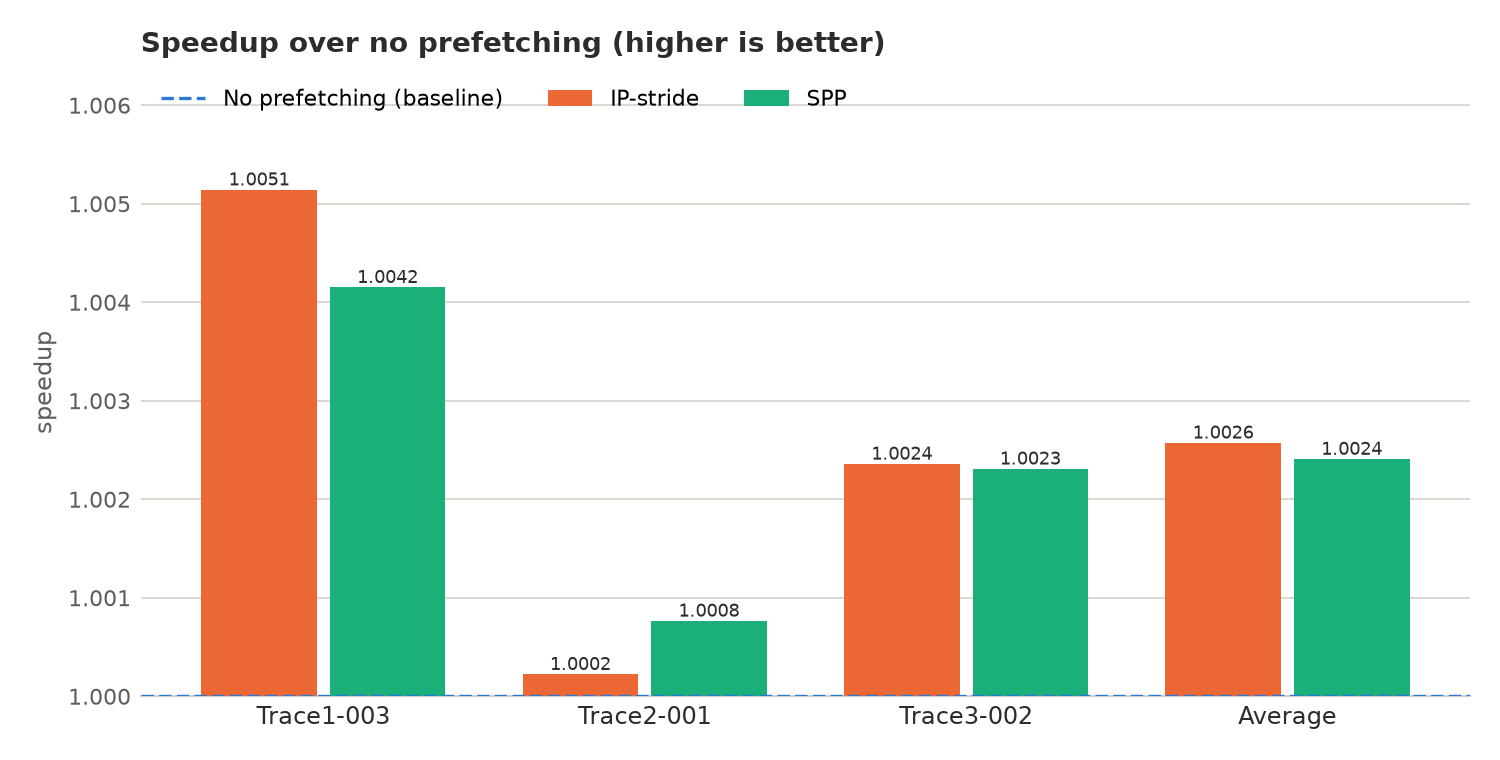
\includegraphics[width=0.49\linewidth]{task1b/plots/speedup.png}\hfill
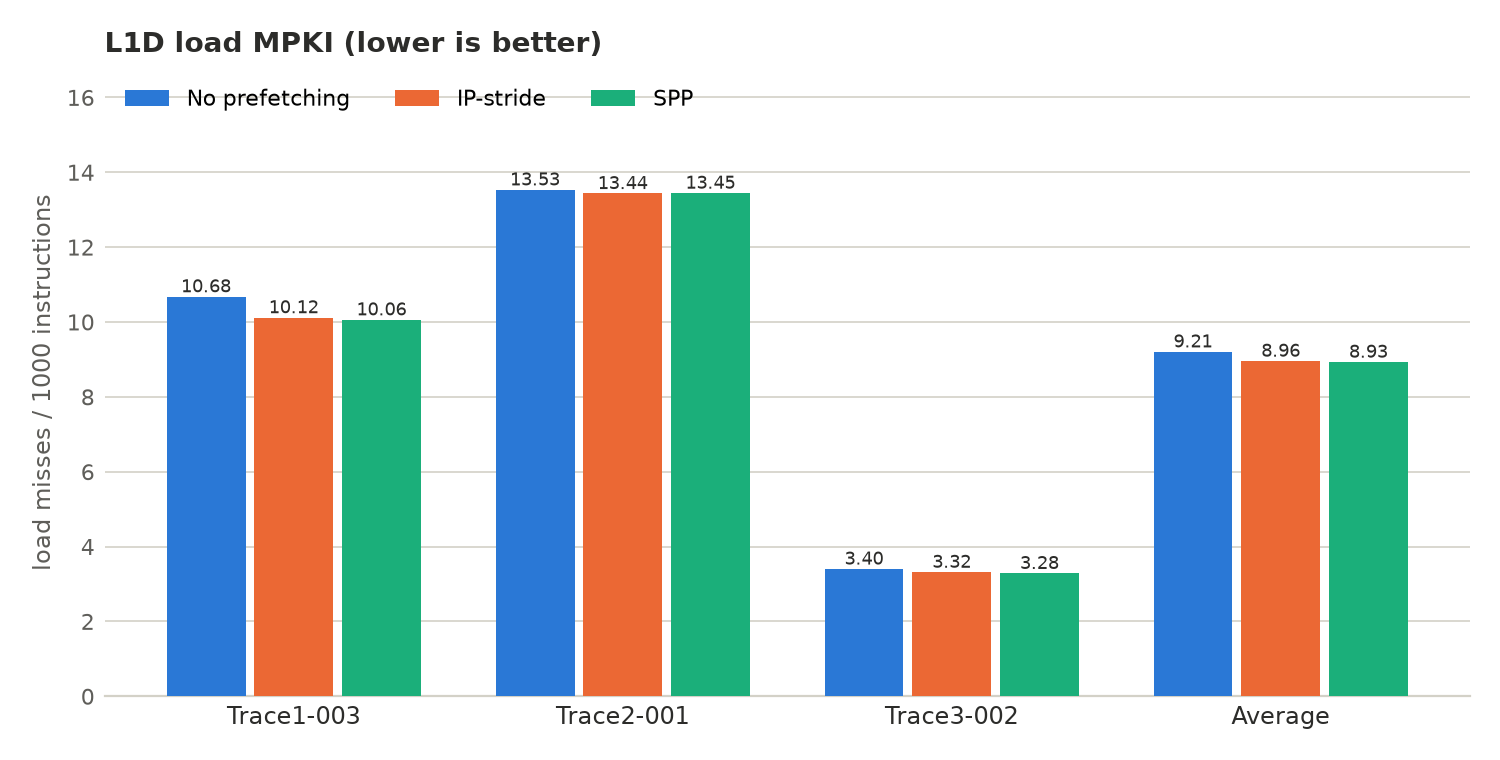
\includegraphics[width=0.49\linewidth]{task1b/plots/mpki.png}\\[0.5em]
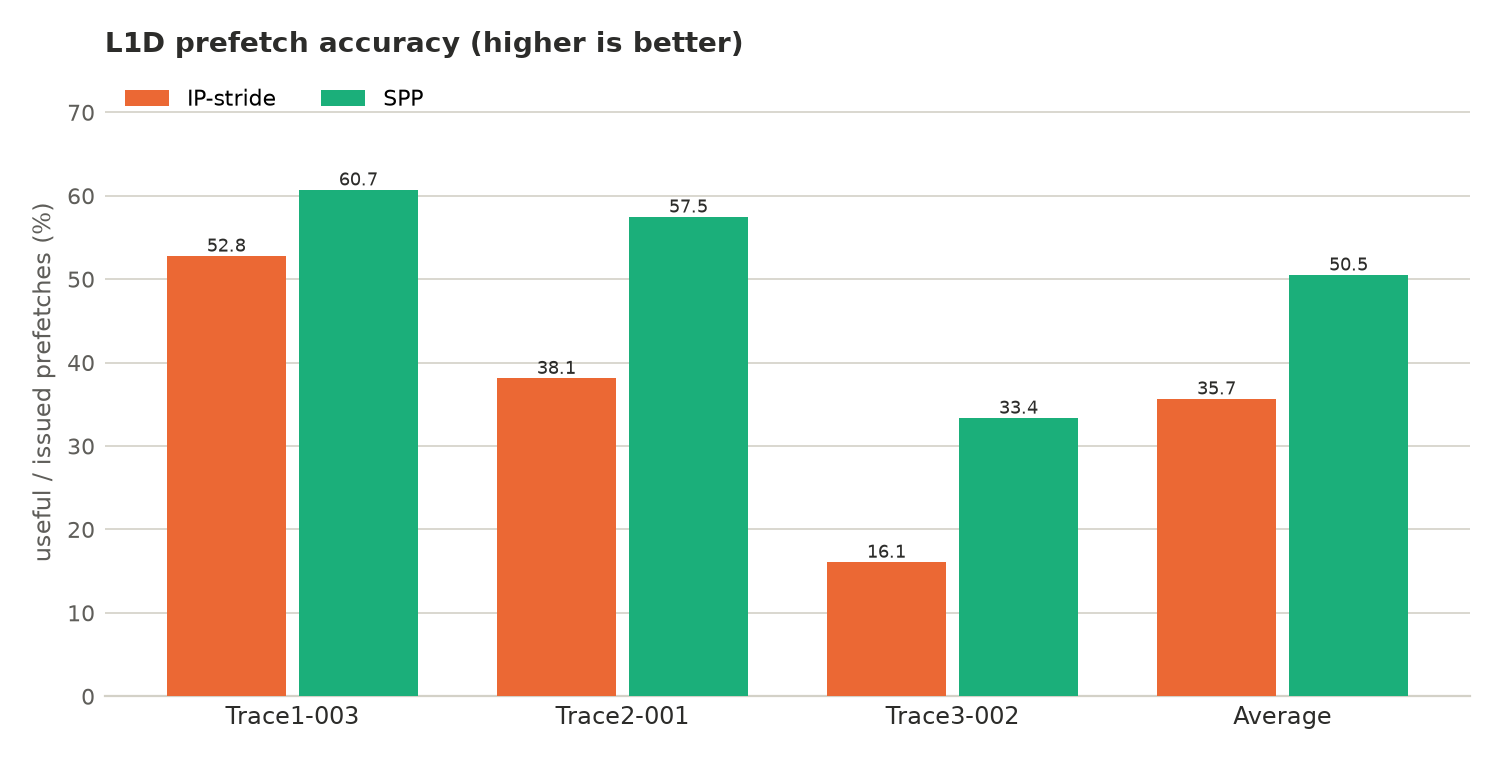
\includegraphics[width=0.49\linewidth]{task1b/plots/accuracy.png}\hfill
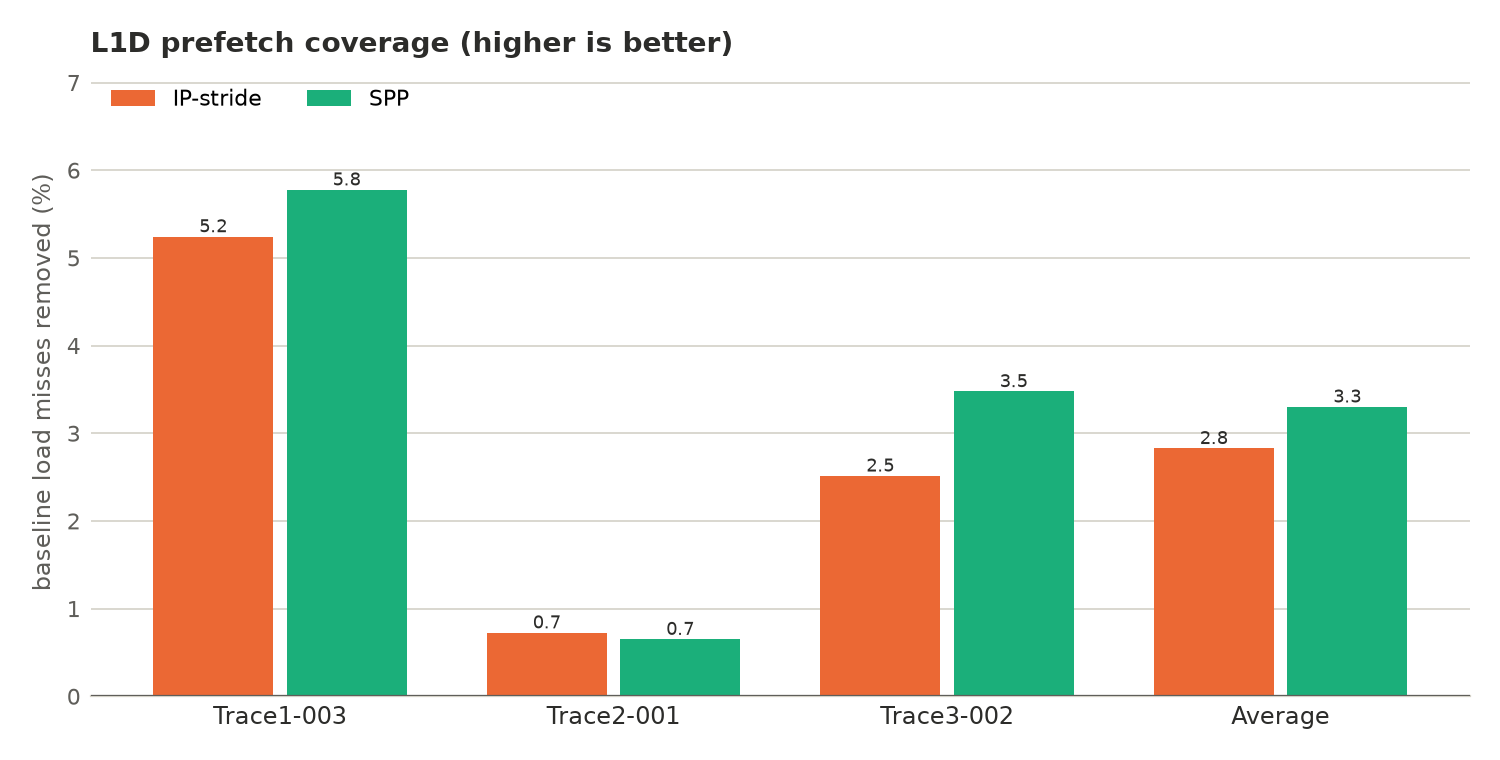
\includegraphics[width=0.49\linewidth]{task1b/plots/coverage.png}
\caption{Speedup, L1D load MPKI, prefetch accuracy and coverage of IP-stride
and SPP.}
\label{fig:t1-metrics}
\end{figure}

\begin{figure}[H]
\centering
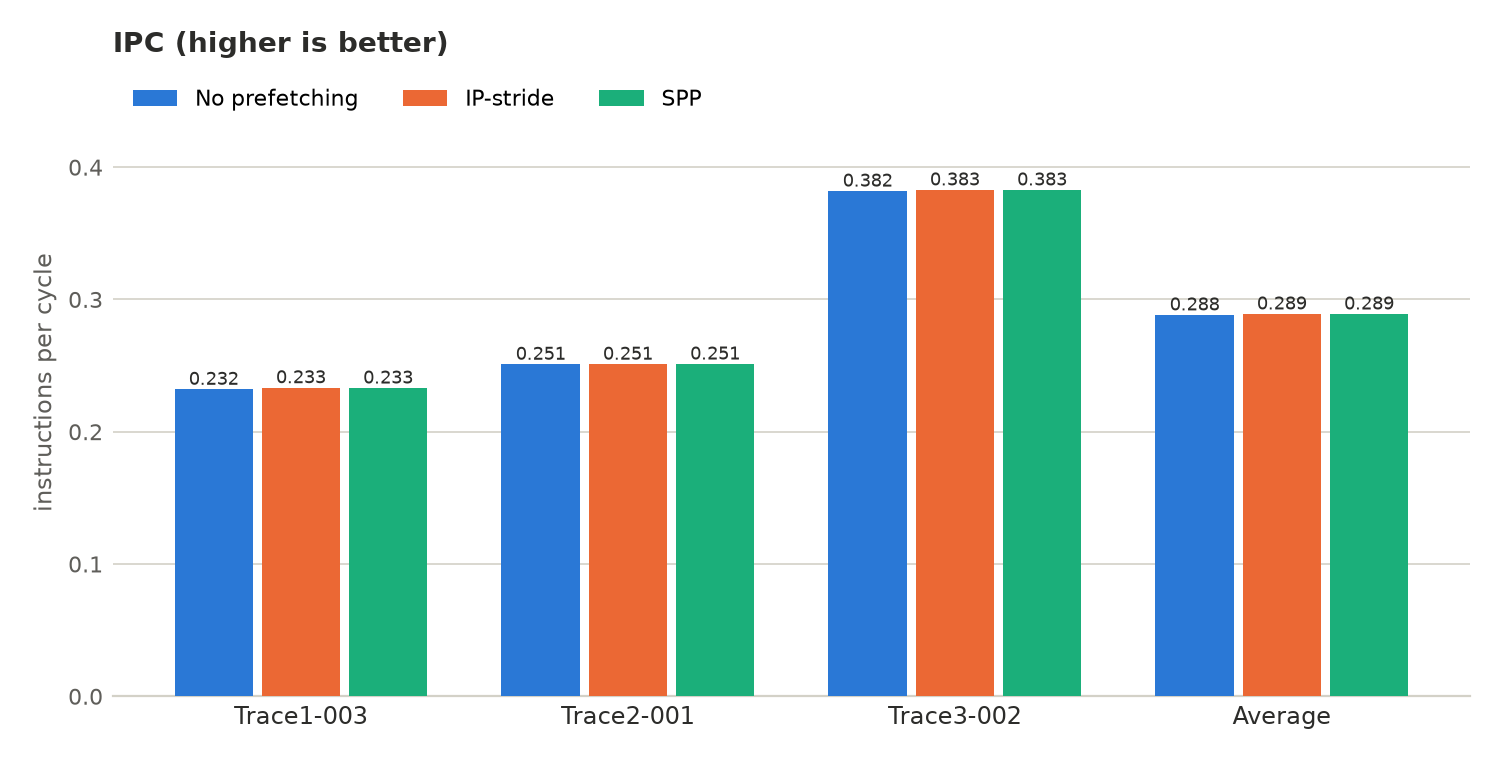
\includegraphics[width=0.6\linewidth]{task1b/plots/ipc.png}
\caption{IPC with no prefetching, IP-stride and SPP.}
\label{fig:t1-ipc}
\end{figure}

\paragraph{Observations.}
\begin{itemize}
  \item \textbf{Accuracy.} SPP is more accurate than IP-stride on every trace
        (50.5\% vs.\ 35.7\% on average). On Trace2 and Trace3 it doubles or
        nearly doubles the accuracy while issuing about half as many prefetches
        (5211 vs.\ 11472 and 9496 vs.\ 17013). The confidence counters and the
        throttle stop SPP from prefetching on strides that do not repeat, which
        IP-stride does after a single repeat with a fixed degree of 3.
  \item \textbf{Coverage and MPKI.} SPP has the higher average coverage
        (3.30\% vs.\ 2.83\%) and the lowest average L1D load MPKI (8.931).
        On Trace1 and Trace3 it turns fewer prefetches into more useful ones
        (e.g.\ 3168 vs.\ 2738 useful on Trace3), which is where the pattern
        predictor adds coverage beyond constant strides. Only on Trace2 is its
        coverage slightly lower (0.65\% vs.\ 0.73\%), because the throttle keeps
        it at a low degree.
  \item \textbf{Speedup.} Both prefetchers give small speedups: 0.26\% (IP-stride)
        and 0.24\% (SPP) geometric mean. SPP is best on Trace2, equal on Trace3
        and slightly behind on Trace1, despite its lower MPKI there. IP-stride
        issues more prefetches and sends them to the L2 when the L1D MSHRs are
        busy, so some of its benefit likely shows up as L2 hits that the L1D
        coverage metric does not count, whereas SPP drops prefetches when fewer
        than 3 MSHRs are free.
  \item \textbf{Why the gains are small.} Coverage is at most 5.8\%: more than
        94\% of the baseline L1D load misses are not predictable from a per-IP
        stride or stride sequence in these traces. Since all three traces have a
        low IPC (0.23--0.38) and the misses that remain dominate execution time,
        removing a few percent of L1D misses changes the IPC very little.
\end{itemize}

\subsection{Storage overhead}

Table~\ref{tab:t1-storage} gives the bit-level breakdown of every table entry
with the field widths used by the implementation. The IP tag is the key of the
IP table and the signature is the key (tag) of the pattern table.

\begin{table}[H]
\centering
\begin{tabular}{llr}
\toprule
Structure & Field & Bits\\
\midrule
IP entry & IP tag (low 8 bits of the IP) & 8\\
         & Last cache-line address & 64\\
         & Stride history / signature ($8 \times 8$-bit strides) & 64\\
         & Monitored (uniform) stride & 8\\
         & Uniform-stride confidence & 8\\
         & LRU age & 8\\
         & \textbf{Total per IP entry (without pattern table)} & \textbf{160}\\
\midrule
Pattern entry & Signature tag ($8 \times 8$-bit strides) & 64\\
              & Next stride & 8\\
              & Confidence & 8\\
              & LRU age & 8\\
              & \textbf{Total per pattern entry} & \textbf{88}\\
\midrule
Per IP & 1 IP entry + 24 pattern entries ($160 + 24 \times 88$) & 2272\\
\midrule
Throttle (global) & Prefetch degree & 32\\
                  & Epoch access counter & 64\\
                  & Snapshot of prefetches issued & 64\\
                  & Snapshot of useful prefetches & 64\\
                  & \textbf{Total} & \textbf{224}\\
\midrule
\multicolumn{2}{l}{\textbf{Total: $24 \times 2272 + 224$}} & \textbf{54752 bits $\approx$ 6.68\,KB}\\
\bottomrule
\end{tabular}
\caption{SPP storage. 24 IP entries, each with a 24-entry pattern table.
The issued/useful counters themselves are ChampSim's existing L1D statistics
and are not counted.}
\label{tab:t1-storage}
\end{table}

Almost all of the storage (93\%) is in the pattern tables. Several fields are
wider than they need to be: the uniform confidence only takes the values 0--2
(2 bits), the pattern confidence never exceeds 127 (7 bits), a cache-line
address of a 64-bit virtual address needs 58 bits, the degree (1--8) fits in
3 bits and the epoch counter (0--255) in 8 bits. With these widths the total
drops to about 6.4\,KB.

\subsection{Choice of throttling thresholds and degrees}

The thresholds and maximum degree were chosen with a sweep on Trace1-003, the
trace with the most prefetch activity (Table~\ref{tab:t1-throttle},
Figures~\ref{fig:t1-thr} and~\ref{fig:t1-deg}). Each run varies the lower
threshold (MIN\_CONF: below it the degree decreases), the upper threshold
(MAX\_CONF: above it the degree increases) or the maximum degree, and is
compared against the no-prefetching baseline of Trace1-003.

\begin{table}[H]
\centering
\small
\setlength{\tabcolsep}{4pt}
\begin{tabular}{rrr rrrrrr}
\toprule
MIN & MAX & Max deg. & IPC & Speedup & MPKI & Acc.\ (\%) & Cov.\ (\%) & PF issued\\
\midrule
0.3 & 0.6  & 4 & 0.2328 & 1.0028 & 10.128 & 62.75 & 5.16 & 24247\\
0.4 & 0.7  & 4 & 0.2328 & 1.0026 & 10.159 & 63.22 & 4.87 & 22478\\
0.5 & 0.75 & 4 & 0.2328 & 1.0025 & 10.193 & 62.50 & 4.54 & 21207\\
0.6 & 0.85 & 4 & 0.2328 & 1.0025 & 10.223 & 62.44 & 4.26 & 19778\\
0.7 & 0.9  & 4 & 0.2327 & 1.0023 & 10.238 & 62.22 & 4.13 & 19167\\
\midrule
0.5 & 0.75 & 2 & 0.2328 & 1.0024 & 10.248 & 61.86 & 4.03 & 18787\\
0.5 & 0.75 & 4 & 0.2328 & 1.0025 & 10.193 & 62.50 & 4.54 & 21207\\
0.5 & 0.75 & 6 & 0.2328 & 1.0027 & 10.159 & 63.02 & 4.86 & 22574\\
0.5 & 0.75 & 8 & 0.2328 & 1.0028 & 10.149 & 63.49 & 4.96 & 22846\\
\bottomrule
\end{tabular}
\caption{SPP throttle sweep on Trace1-003 (MIN/MAX = MIN\_CONF/MAX\_CONF, MPKI = L1D load MPKI). Top: threshold pairs at maximum
degree 4. Bottom: maximum degree at thresholds 0.5/0.75.}
\label{tab:t1-throttle}
\end{table}

\begin{figure}[H]
\centering
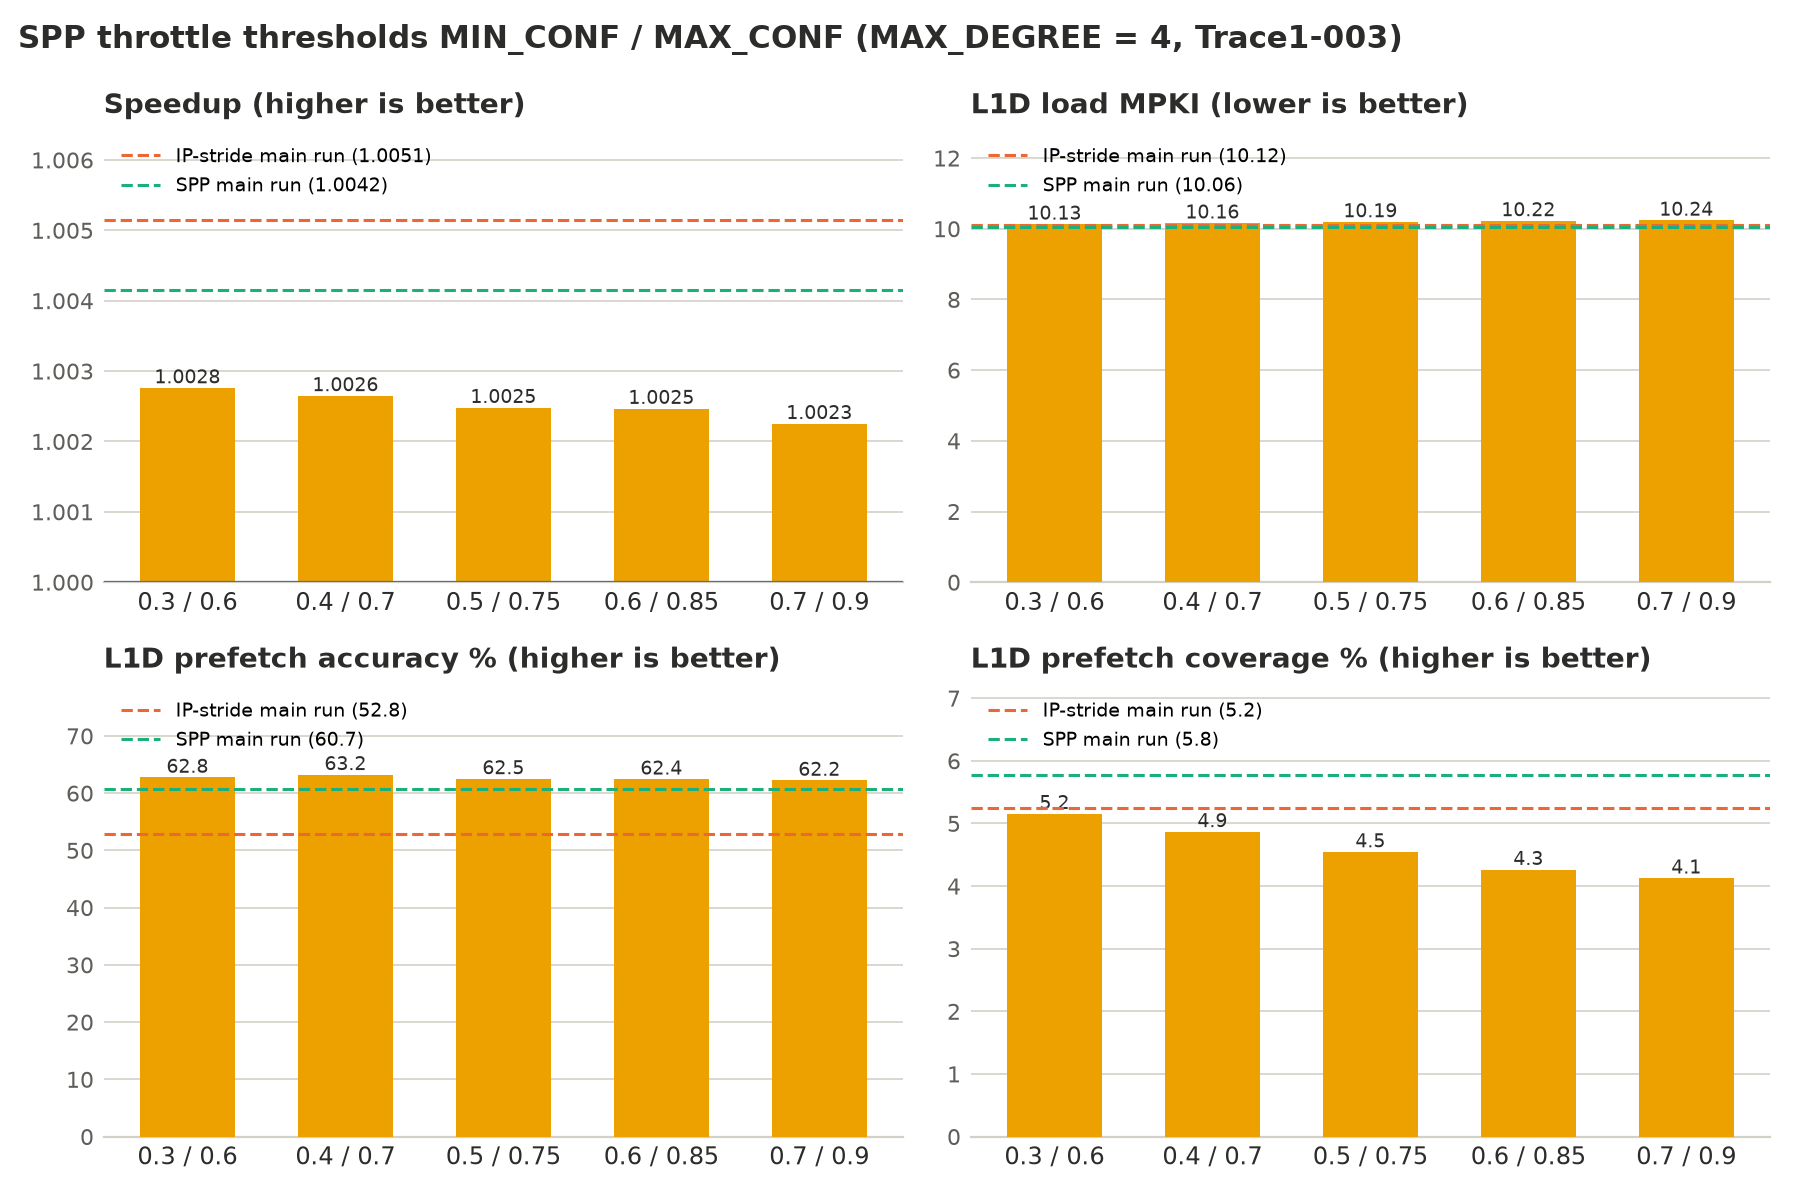
\includegraphics[width=0.85\linewidth]{task1b/plots/throttle_thresholds.png}
\caption{Sweep over the accuracy thresholds (maximum degree 4).}
\label{fig:t1-thr}
\end{figure}

\begin{figure}[H]
\centering
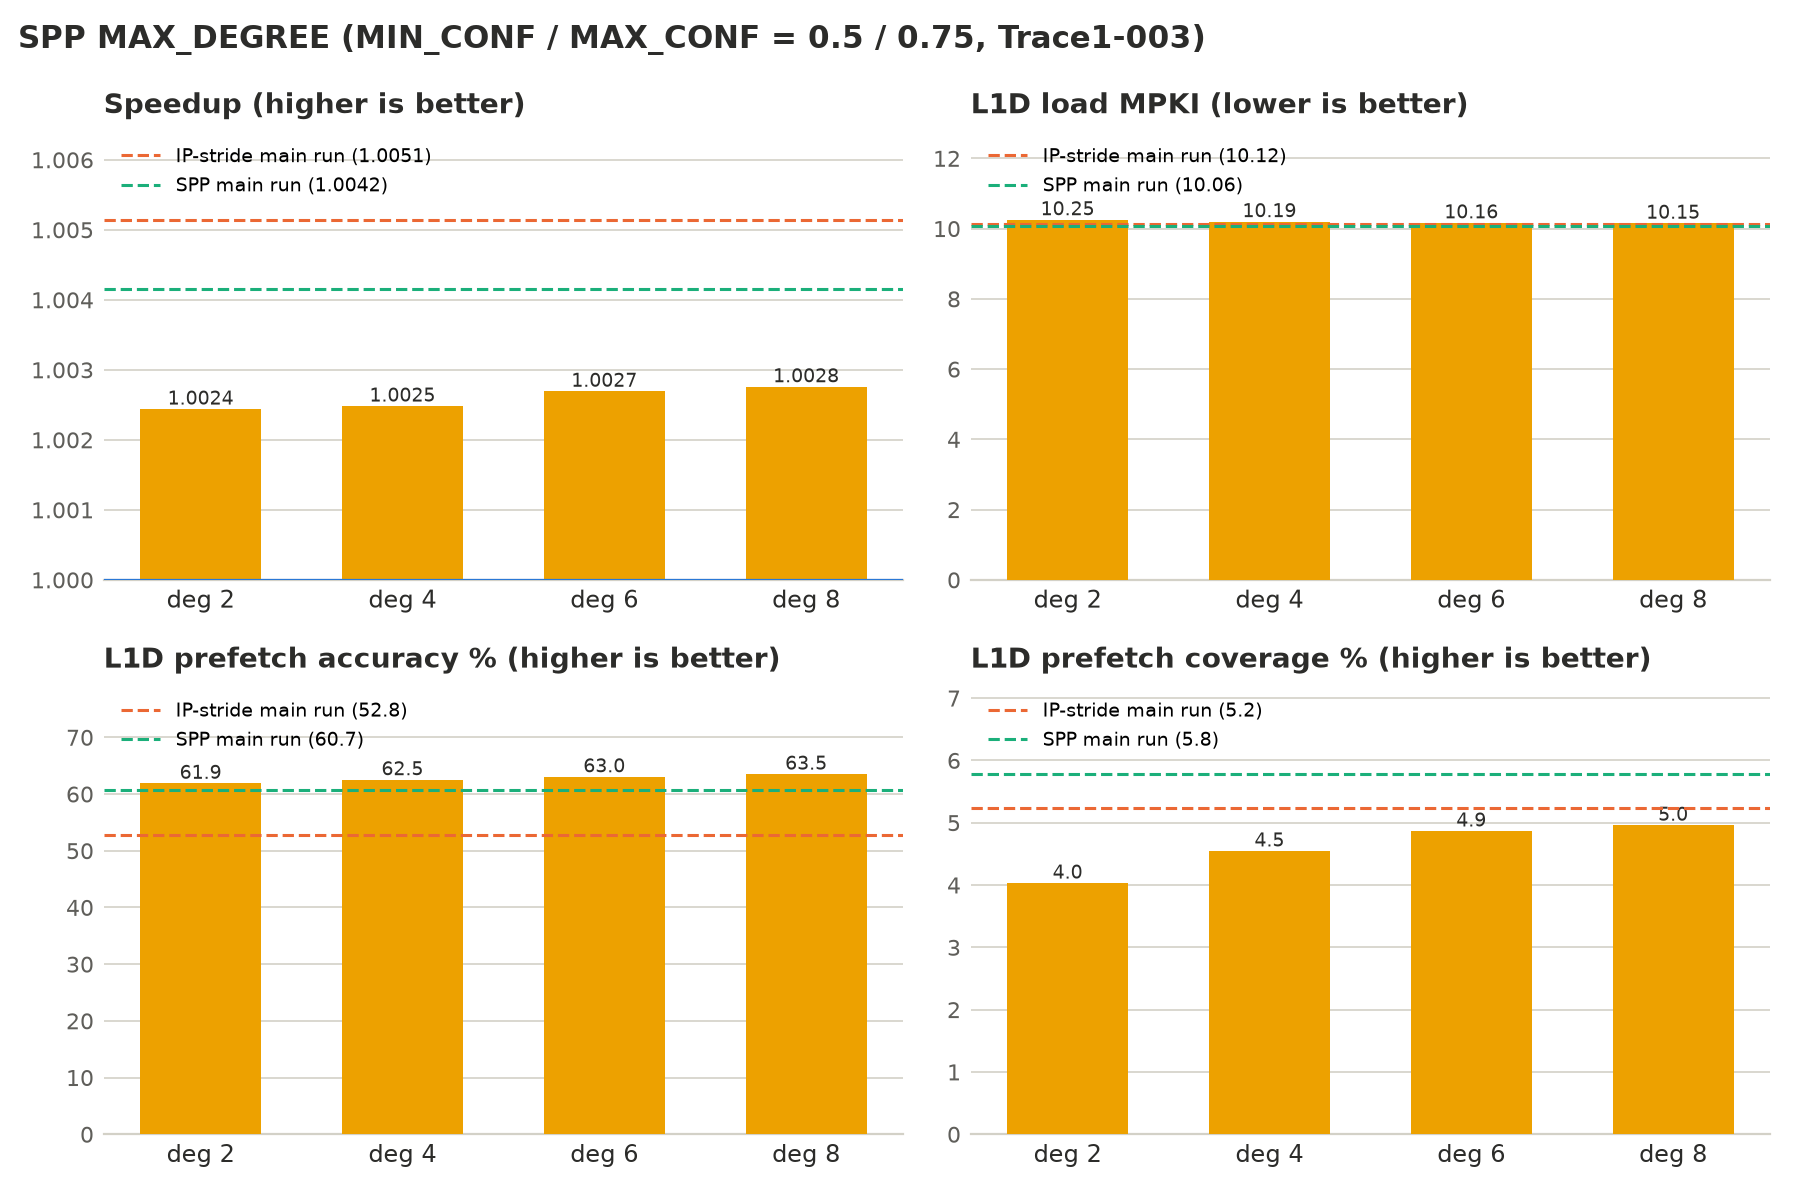
\includegraphics[width=0.85\linewidth]{task1b/plots/throttle_degree.png}
\caption{Sweep over the maximum degree (thresholds 0.5/0.75).}
\label{fig:t1-deg}
\end{figure}

\paragraph{How the thresholds were decided.}
SPP's epoch accuracy on this trace sits around 62--63\% for every setting.
With high thresholds (e.g.\ 0.7/0.9) that accuracy is rarely above MAX\_CONF,
so the degree seldom grows, and it is often below MIN\_CONF, so the degree is
pulled down; SPP issues fewer prefetches (19167) and coverage falls to 4.13\%.
Lowering the thresholds increases the speedup monotonically, from 1.0023 at
0.7/0.9 to 1.0028 at 0.3/0.6, and coverage rises from 4.13\% to 5.16\%, while
accuracy does not drop (62.2\% $\to$ 62.8\%). The extra prefetches are as
useful as the rest, so being more aggressive does not cause pollution here.
We therefore use \textbf{MIN\_CONF = 0.3} and \textbf{MAX\_CONF = 0.6}:
\begin{itemize}
  \item Accuracy above 60\%: more than every second prefetch is used, so
        prefetching further ahead is worth the bandwidth; the degree grows.
  \item Accuracy between 30\% and 60\%: the prefetches still help but are not
        reliable enough to issue more of them; the degree is kept.
  \item Accuracy below 30\%: more than two out of three prefetches are wasted
        and only pollute the L1D and occupy MSHRs; the degree shrinks, down to 1.
\end{itemize}
We did not go below 0.3/0.6: the low threshold is the only protection against
pollution on phases or traces where the patterns break down (Trace3 has an
accuracy of only 33\%), and on traces like that a lower threshold would leave
SPP running at a high degree with mostly useless prefetches.

\paragraph{Why these degrees.}
The degree starts at 1, so an IP's first predictions are cheap, and changes by
one step per epoch, so a single noisy epoch cannot swing it far. At thresholds
0.5/0.75 raising the maximum degree from 2 to 8 increases the speedup
monotonically (1.0024 $\to$ 1.0028), coverage (4.03\% $\to$ 4.96\%) and even
accuracy (61.9\% $\to$ 63.5\%): when patterns are confident, prefetching further
ahead hides more of the miss latency without polluting the cache. We use
\textbf{a maximum degree of 8}. A larger maximum is of limited use because a
prefetch never crosses the 4\,KB page (64 lines): at strides of a few lines,
8 steps already reach much of the page, and the remaining targets would be
dropped anyway. The minimum degree of 1 keeps SPP training and measuring its
accuracy even in bad phases, so it can raise the degree again once its
prefetches become useful.

The final configuration (0.3/0.6, maximum degree 8) combines the best setting
from each sweep. With it, SPP reaches a speedup of 1.0042 on Trace1-003, higher
than any setting in the sweep, with 60.7\% accuracy and 5.78\% coverage
(Table~\ref{tab:t1-pf}). The sweep was run only on Trace1-003 and before the
final runs, so its absolute numbers are best compared with each other rather
than with the main results.


%======================================================================
\section{Task 2A: Instruction-Conscious L2 Replacement (I-RRIP)}

Policy file: \texttt{replacement/irrip.l2c\_repl}.

\subsection{In short}
\begin{itemize}
  \item The L2 cache holds both program code (instruction lines) and data. When
        it is full, the replacement policy decides which line to evict.
  \item I-RRIP tries harder to keep instruction lines, because when code is
        missing the CPU cannot even fetch its next instruction.
  \item Result: fewer L2 instruction misses on every trace, and on the
        code-heavy trace (Trace2) the program runs 2.4\% faster than with LRU.
        Average over the three traces: 0.79\% faster.
\end{itemize}

\subsection{Telling the policy ``code or data?''}
Originally the replacement policy had no way to know whether a line held code
or data. We added one extra input, \texttt{isInstruction}, to
\texttt{update\_replacement\_state()}, which the cache calls on every hit and
every fill. It is 1 for an instruction line and 0 for everything else. Because
all caches share this function's signature, the input was added everywhere it is
declared, defined and called.

The value is computed by a small helper in \texttt{cache.cc}: a request is an
instruction line only when it is a normal read (LOAD) or a PREFETCH and its
\texttt{packet.instruction} flag is set. This is the same rule the simulator
already uses to mark L2 lines as instruction lines, so address-translation
lookups and writebacks are never mistaken for code.

\subsection{The policy}
I-RRIP starts from SRRIP (\texttt{rrip.l2c\_repl}). Every line has a 2-bit
re-reference prediction value (RRPV) from 0 to 3: 0 = ``will be used again
soon, keep me'', 3 = ``not needed soon, evict me first''. I-RRIP changes how
these values are assigned and used so that code lines stay longer
(Table~\ref{tab:t2a-rules}; the reasoning is in Section~\ref{sec:t2a-design}).

\begin{table}[H]
\centering
\begin{tabular}{lll}
\toprule
Part & SRRIP & I-RRIP\\
\midrule
Insertion, instruction line & RRPV 2 & RRPV 1\\
Insertion, data line & RRPV 2 & RRPV 2\\
Promotion (hit), instruction line & RRPV 0 & RRPV 0\\
Promotion (hit), data line & RRPV 0 & RRPV 1\\
Promotion on a writeback hit & RRPV 0 & no change\\
Eviction & first line at RRPV 3 & first data line at RRPV 3,\\
         &                      & then any line at RRPV 3\\
Empty way in the set & not checked & used first\\
\bottomrule
\end{tabular}
\caption{SRRIP vs.\ I-RRIP rules. A hit never raises a line's RRPV.}
\label{tab:t2a-rules}
\end{table}

\subsection{Experimental setup}
\begin{itemize}
  \item 25M warmup + 25M measured instructions on each of the three traces.
  \item No L1D prefetcher; every other cache uses LRU. The baseline is LRU at
        the L2 (1024 sets $\times$ 8 ways, 512\,KB).
  \item Speedup = IPC with the policy / IPC with LRU, on the same trace. The
        average is the geometric mean.
  \item MPKI = misses per 1000 instructions (lower is better). We report the
        L2C load MPKI and its two parts: instruction and data.
  \item The simulator is deterministic (fixed random seeds), so one run per
        setting is enough. Re-running from the final code gave identical
        results.
\end{itemize}

\subsection{Results}

\begin{table}[H]
\centering
\begin{tabular}{llrrrrr}
\toprule
Trace & Policy & IPC & Speedup & L2C load & L2 instr. & L2 data\\
      &        &     &         & MPKI     & MPKI      & MPKI\\
\midrule
Trace1 & LRU (baseline) & 0.2323 & 1.0000 & 17.696 & 10.338 & 7.358\\
       & SRRIP          & 0.2322 & 0.9995 & 17.639 & 10.562 & 7.077\\
       & I-RRIP         & 0.2322 & 0.9994 & 17.649 &  9.765 & 7.884\\
\midrule
Trace2 & LRU (baseline) & 0.2512 & 1.0000 & 27.357 & 18.853 & 8.504\\
       & SRRIP          & 0.2518 & 1.0026 & 25.746 & 17.781 & 7.965\\
       & I-RRIP         & 0.2572 & 1.0241 & 21.329 & 12.204 & 9.125\\
\midrule
Trace3 & LRU (baseline) & 0.3821 & 1.0000 &  3.954 &  1.124 & 2.830\\
       & SRRIP          & 0.3817 & 0.9991 &  4.039 &  1.197 & 2.842\\
       & I-RRIP         & 0.3822 & 1.0003 &  3.823 &  0.957 & 2.866\\
\midrule
Average & LRU (baseline) & & 1.0000 & & & \\
        & SRRIP          & & 1.0004 & & & \\
        & I-RRIP         & & 1.0079 & & & \\
\bottomrule
\end{tabular}
\caption{Task 2A: IPC, speedup over LRU, and L2 load misses per 1000 instructions.}
\label{tab:t2a-results}
\end{table}

\begin{table}[H]
\centering
\begin{tabular}{lrrrr}
\toprule
Trace & L2 instr.\ MPKI & L2 data MPKI & L2C load MPKI & Speed\\
\midrule
Trace1 &  $-5.5\%$ & $+7.2\%$ &  $-0.3\%$ & $-0.06\%$\\
Trace2 & $-35.3\%$ & $+7.3\%$ & $-22.0\%$ & $+2.41\%$\\
Trace3 & $-14.9\%$ & $+1.3\%$ &  $-3.3\%$ & $+0.03\%$\\
\bottomrule
\end{tabular}
\caption{Change of each metric with I-RRIP relative to LRU (negative MPKI change = fewer misses).}
\label{tab:t2a-delta}
\end{table}

\begin{figure}[H]
\centering
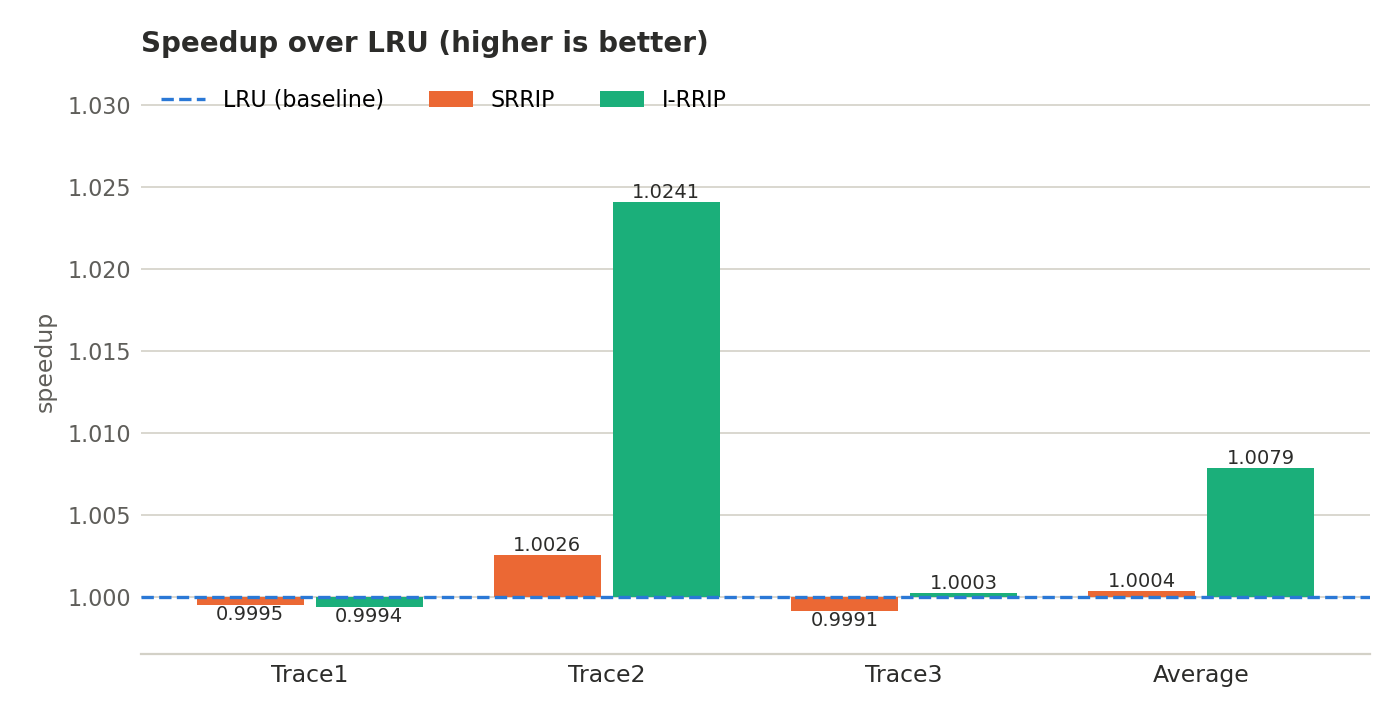
\includegraphics[width=0.49\linewidth]{task2a/plots/speedup.png}\hfill
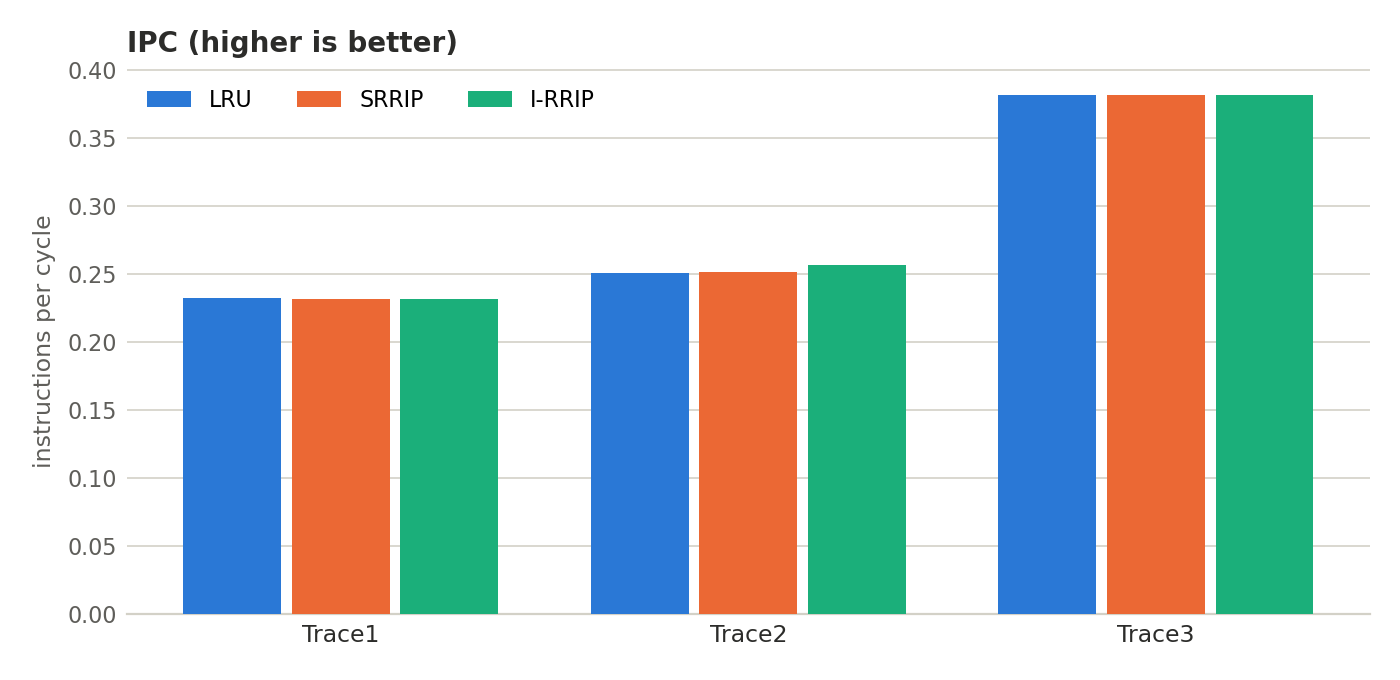
\includegraphics[width=0.49\linewidth]{task2a/plots/ipc.png}
\caption{Task 2A: speedup over LRU (dashed line: LRU = 1.0) and IPC per trace.}
\label{fig:t2a-speedup}
\end{figure}

\begin{figure}[H]
\centering
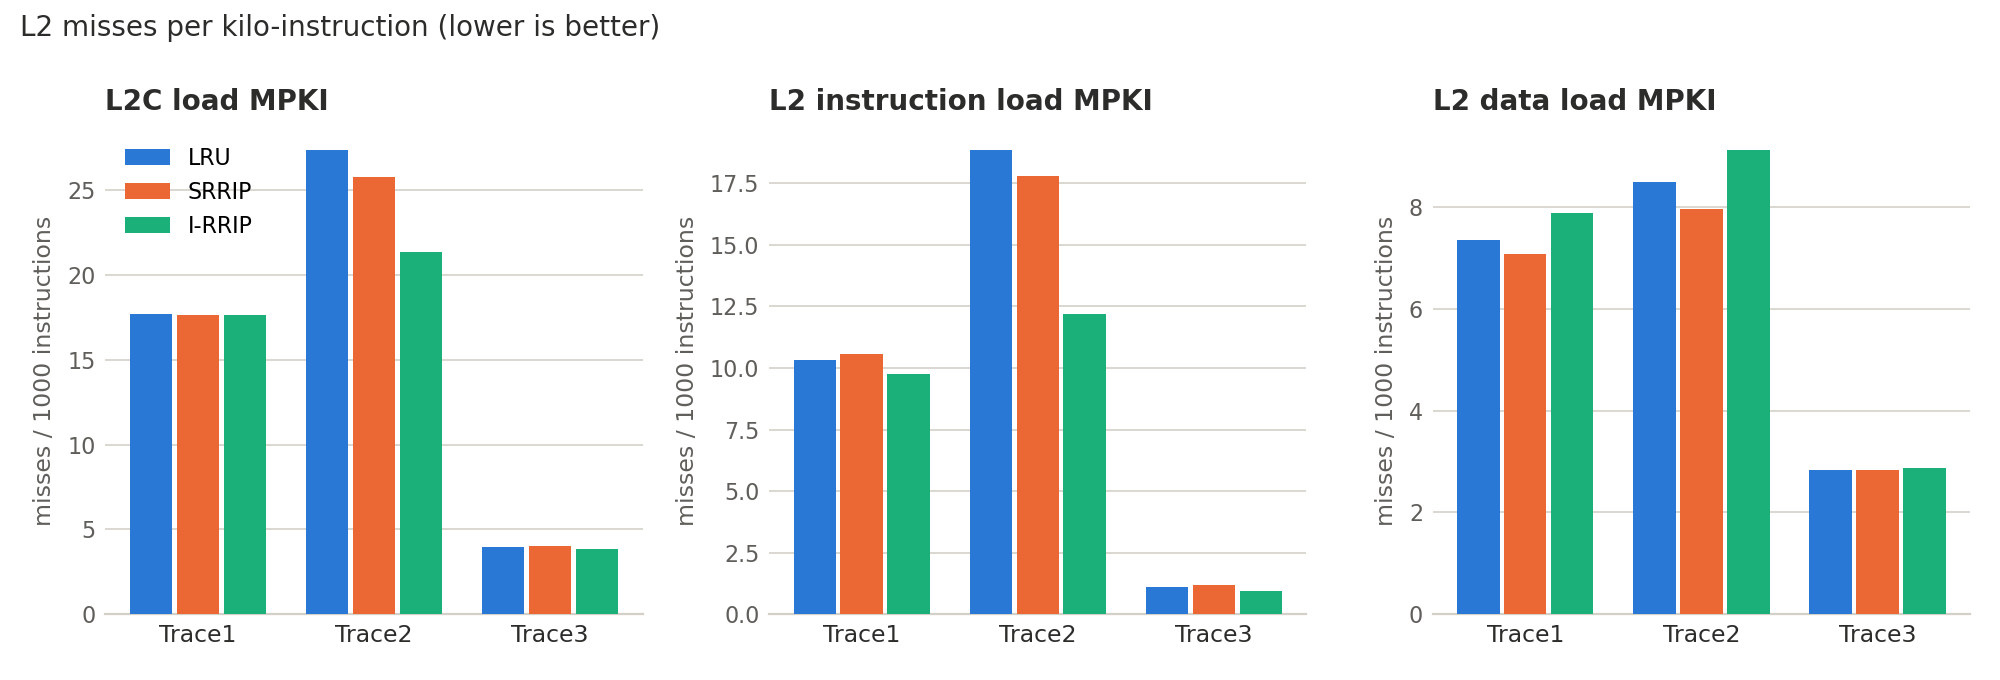
\includegraphics[width=0.9\linewidth]{task2a/plots/mpki.png}
\caption{Task 2A: L2 misses per 1000 instructions: all loads, instruction loads, data loads.}
\label{fig:t2a-mpki}
\end{figure}

\paragraph{Observations.}
\begin{itemize}
  \item \textbf{The goal is met.} I-RRIP lowers L2 instruction misses on every
        trace: $-5.5\%$ (Trace1), $-35.3\%$ (Trace2) and $-14.9\%$ (Trace3).
  \item \textbf{Trace2 gains the most.} It has many more code misses than data
        misses (18.85 vs.\ 8.50 MPKI with LRU). There I-RRIP removes 22\% of all
        L2 load misses and runs 2.4\% faster.
  \item \textbf{The price is a few more data misses}, because data lines are now
        evicted earlier. On Trace1 and Trace3 code misses were already low, so
        the small gain and the small loss cancel out and the speed stays the
        same (within 0.1\%).
  \item \textbf{SRRIP alone hardly helps} (average speedup 1.0004). The
        improvement comes from treating code lines differently.
\end{itemize}

\subsection{Design choices}
\label{sec:t2a-design}
We changed all three parts of the policy: insertion (RRPV of a new line),
promotion (RRPV after a hit) and eviction (which line to evict). To check that
each change is useful, we also ran the policy with only one change enabled at a
time, using the same binary with different settings
(Table~\ref{tab:t2a-ablation}, Figure~\ref{fig:t2a-variants}).

\begin{table}[H]
\centering
\small
\setlength{\tabcolsep}{3.5pt}
\begin{tabular}{lrrrr}
\toprule
Version & Avg.\ speedup & Trace2 speedup & Trace2 instr.\ MPKI & Trace2 data MPKI\\
\midrule
LRU (baseline)                          & 1.0000 & 1.0000 & 18.853 & 8.504\\
SRRIP                                   & 1.0004 & 1.0026 & 17.781 & 7.965\\
Only the two small fixes (\S\ref{sec:t2a-fixes}) & 1.0039 & 1.0111 & 15.619 & 7.873\\
\quad + promotion change only           & 1.0051 & 1.0149 & 14.478 & 8.376\\
\quad + insertion change only           & 1.0054 & 1.0155 & 14.711 & 8.363\\
\quad + eviction change only            & 1.0080 & 1.0236 & 12.653 & 8.428\\
All, but new code at RRPV 0             & 1.0072 & 1.0229 & 12.525 & 9.274\\
\textbf{I-RRIP (all three)}             & \textbf{1.0079} & \textbf{1.0241} & \textbf{12.204} & 9.125\\
\bottomrule
\end{tabular}
\caption{Each change on its own. All variants except LRU and SRRIP include the two small fixes.}
\label{tab:t2a-ablation}
\end{table}

\begin{figure}[H]
\centering
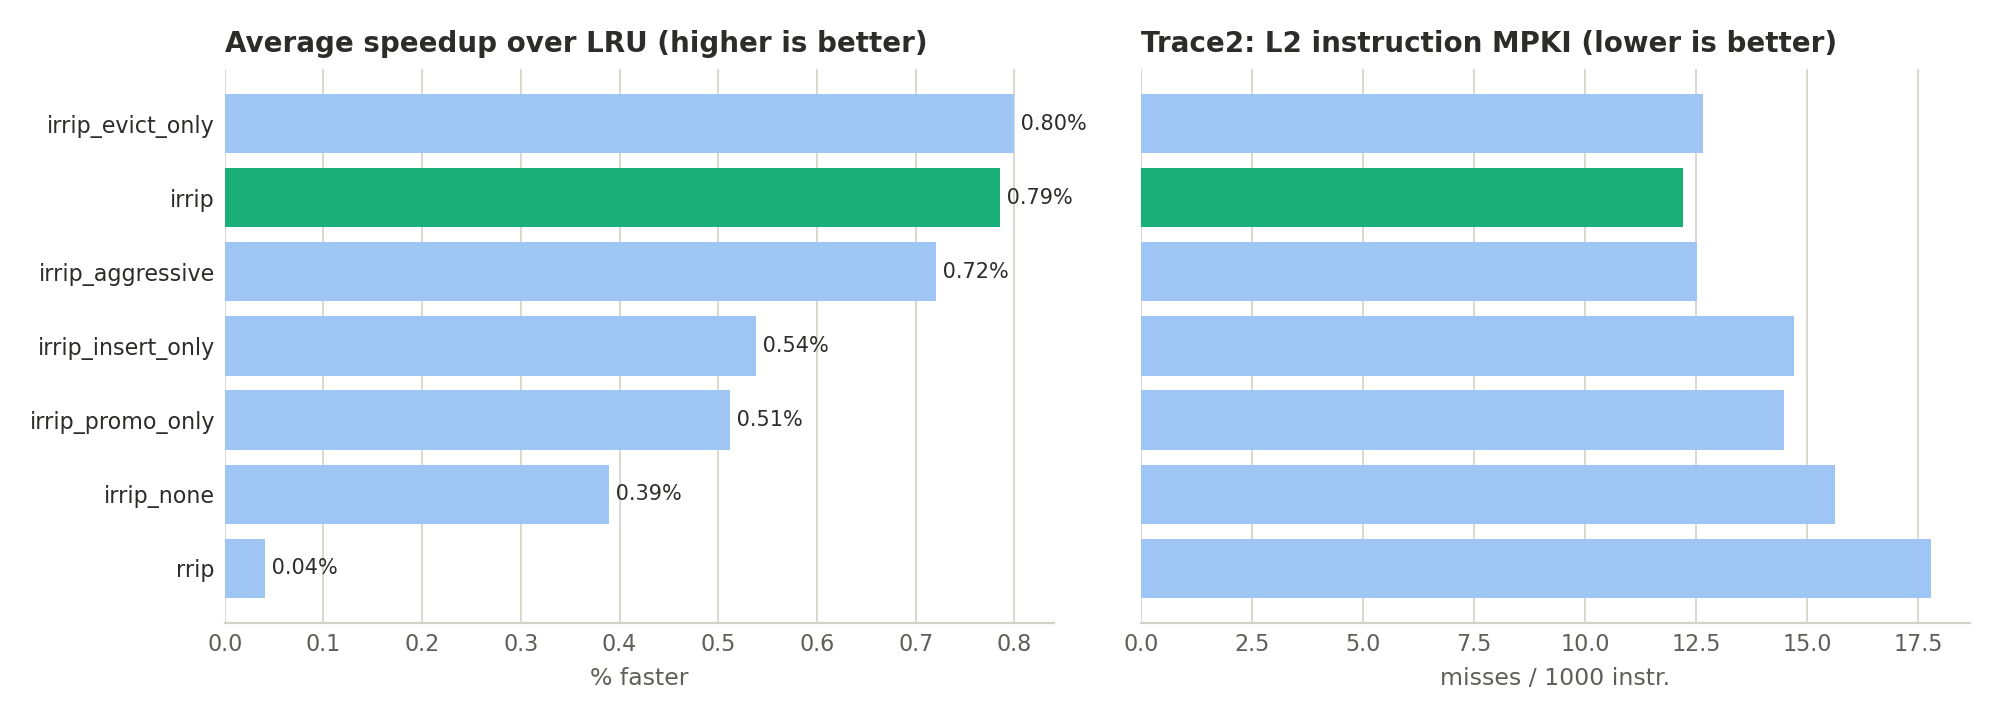
\includegraphics[width=0.9\linewidth]{task2a/plots/variants.png}
\caption{The comparison of Table~\ref{tab:t2a-ablation} as a chart; I-RRIP is
green. \texttt{irrip\_none} = only the two small fixes;
\texttt{irrip\_promo\_only} / \texttt{irrip\_insert\_only} /
\texttt{irrip\_evict\_only} = one change only; \texttt{irrip\_aggressive} = new
code at RRPV 0.}
\label{fig:t2a-variants}
\end{figure}

\paragraph{Insertion: new code lines at RRPV 1, new data lines at RRPV 2.}
SRRIP inserts every new line at RRPV 2. A code line inserted at 1 gets one
extra round before it can be evicted, so it has more time to be reused, while
data is not hurt more than needed. We did not use RRPV 0 for code: then code
that runs only once (e.g.\ start-up code) would be protected as much as code
that is used again and again. Evidence: with RRPV 0, data misses go up (9.27
vs.\ 9.13 MPKI on Trace2), code misses do not go down, and the average speedup
is lower (1.0072 vs.\ 1.0079). On its own, this change raises the Trace2
speedup from 1.0111 to 1.0155.

\paragraph{Promotion: a reused code line goes to RRPV 0, a reused data line only to RRPV 1.}
With SRRIP, popular data competes equally with popular code. Now code that is
reused always ranks above data that is reused. A hit never makes a line's RRPV
worse. On its own, this change raises the Trace2 speedup from 1.0111 to 1.0149
and lowers code misses from 15.62 to 14.48 MPKI.

\paragraph{Eviction: data before code.}
When a line must be evicted, we first look for a data line at RRPV 3; only if
there is none do we take a code line at RRPV 3. If no line is at RRPV 3, all
RRPVs are incremented and the search repeats. Among lines that are ``not needed
soon'', losing a data line usually hurts less than losing a code line. This is
the strongest single change: on its own it gives an average speedup of 1.0080
and cuts Trace2 code misses from 18.85 (LRU) to 12.65 MPKI.

\paragraph{Two small fixes (not about code vs.\ data).}
\label{sec:t2a-fixes}
\begin{itemize}
  \item \textbf{Use an empty way first.} If a way in the set is empty, it is
        used instead of evicting a line. SRRIP's search did not check this.
  \item \textbf{Writebacks do not count as reuse.} A writeback is the L1D
        pushing a modified line down, not the program reading it again. SRRIP
        still set such lines to RRPV 0; we leave their RRPV unchanged (the
        repository's LRU policy does the same).
\end{itemize}
These two alone give an average speedup of 1.0039 (SRRIP: 1.0004). The three
code-vs-data changes then take it to 1.0079.

\paragraph{Why this combination.}
\begin{itemize}
  \item It has the fewest L2 instruction misses on the code-heavy trace: 12.20
        MPKI, $-35.3\%$ compared with LRU, which is exactly what Task 2A asks for.
  \item It is the fastest on Trace2 (1.0241) and its average speedup (1.0079)
        is within 0.01\% of the best single change (eviction only, 1.0080).
  \item Each of the three changes helps on its own, and the one alternative we
        tried for insertion (RRPV 0) was worse.
  \item Limitation: on traces with few code misses (Trace1, Trace3) the
        trade-off brings no gain. Enabling it only when code matters is the idea
        of Task 2B.
\end{itemize}

\subsection{Storage overhead}

\begin{table}[H]
\centering
\begin{tabular}{ll}
\toprule
Stored state & Size (L2: 1024 sets $\times$ 8 ways = 8192 lines)\\
\midrule
RRPV, 2 bits per line (same as SRRIP) & $8192 \times 2$ bits = 2\,KB\\
Instruction bit, 1 bit per line & $8192 \times 1$ bit = 1\,KB\\
\midrule
\textbf{Total} & \textbf{3\,KB}\\
\bottomrule
\end{tabular}
\caption{Storage needed by I-RRIP: 0.6\% of the 512\,KB cache and 1\,KB more than SRRIP.}
\label{tab:t2a-storage}
\end{table}

%======================================================================
\section{Task 2B: Dynamic I-RRIP (Set Dueling)}

Policy file: \texttt{replacement/dyn\_irrip.l2c\_repl}.

\subsection{In short}
\begin{itemize}
  \item I-RRIP (Task 2A) always protects instruction lines. That is good when
        code misses dominate, but in a phase where data matters more it evicts
        data early for nothing.
  \item Dynamic I-RRIP decides at run time. A few \emph{leader} sets always run
        plain SRRIP and measure how much of the L2 traffic is instruction
        traffic. If that share is above a threshold, all other sets
        (\emph{followers}) use I-RRIP; otherwise they use SRRIP.
  \item Result: 2.23\% faster than LRU on Trace2 (code-heavy) and 0.68\% faster
        on average, with 33\% fewer L2 instruction misses on Trace2. It keeps
        about 87\% of the I-RRIP gain while being able to step back to SRRIP
        when code stops mattering.
\end{itemize}

\subsection{Design}

\paragraph{Leader and follower sets.}
Of the 1024 L2 sets, 32 are leader sets (about 3\% of the cache). Leader sets
always use plain SRRIP: insert at RRPV 2, set RRPV 0 on a hit, evict the first
line at RRPV 3. The other 992 sets are followers and use whichever mode the
leaders last chose: I-RRIP (exactly the Task 2A rules) or SRRIP. The leaders are
spread over the whole cache, one in every block of 32 sets, at a position that
moves by one in each block (sets 0, 33, 66, \ldots, 1023), so they do not all
share the same low index bits.

\paragraph{What the leaders count.}
In a leader set, every L2 access that is not a writeback updates four counters:
instruction accesses, instruction misses, total accesses and total misses. A hit
counts as one access; a fill (i.e.\ a miss) counts as one access and one miss.
Instruction lines are recognised with the \texttt{isInstruction} input added in
Task 2A. Writebacks are skipped because they are the L1D evicting dirty lines,
not the program asking for anything.

\paragraph{The decision.}
Every 1024 leader accesses (one \emph{window}) the policy computes the ratio
from the assignment:
\[
  \text{ratio} = \frac{\text{instr.\ accesses} + \text{instr.\ misses}}
                      {\text{total accesses} + \text{total misses}}
\]
If $\text{ratio} > \text{threshold}$ (default 0.25), followers use I-RRIP;
otherwise SRRIP. The ratio is the share of L2 work caused by code, with misses
counted twice because a miss costs much more than a hit. After each decision the
counters are halved, so they keep a memory of about the last two windows.

\paragraph{Follower sets.}
A follower in I-RRIP mode applies all three Task 2A rules (insertion,
promotion including the writeback rule, and data-first eviction). In SRRIP mode
it behaves exactly like a leader. Both modes use an empty way first. Because
the RRPV bits mean the same in both modes, switching needs no reset: lines keep
their RRPVs and the new rules apply from the next access.

\subsection{Experimental setup}
\begin{itemize}
  \item Same setup as Task 2A: 25M warmup + 25M measured instructions per
        trace, no L1D prefetcher, LRU in every other cache, baseline = LRU at
        the L2. Speedup = IPC / IPC(LRU); averages are geometric means.
  \item All settings (threshold, number of leaders, window) are read from
        environment variables (\texttt{DYN\_THRESHOLD}, \texttt{DYN\_LEADERS},
        \texttt{DYN\_WINDOW}), so the sensitivity runs use one binary and
        differ only in the setting being studied. Runner:
        \texttt{scripts/run\_task2b.sh}; tables and plots:
        \texttt{scripts/parse\_results.py}, \texttt{plot\_results.py},
        \texttt{plot\_task2b.py}.
  \item The policy prints its own statistics after warmup: number of decisions,
        mode switches, average ratio and the share of follower accesses served
        in I-RRIP mode.
\end{itemize}

\subsection{Results (threshold 0.25, 32 leader sets)}

\begin{table}[H]
\centering
\begin{tabular}{llrrrrr}
\toprule
Trace & Policy & IPC & Speedup & L2C load & L2 instr. & L2 data\\
      &        &     &         & MPKI     & MPKI      & MPKI\\
\midrule
Trace1 & LRU (baseline)   & 0.2323 & 1.0000 & 17.696 & 10.338 & 7.358\\
       & SRRIP            & 0.2322 & 0.9995 & 17.639 & 10.562 & 7.077\\
       & I-RRIP (Task 2A) & 0.2322 & 0.9994 & 17.649 &  9.765 & 7.884\\
       & Dyn-I-RRIP       & 0.2321 & 0.9991 & 17.651 &  9.788 & 7.864\\
\midrule
Trace2 & LRU (baseline)   & 0.2512 & 1.0000 & 27.357 & 18.853 & 8.504\\
       & SRRIP            & 0.2518 & 1.0026 & 25.746 & 17.781 & 7.965\\
       & I-RRIP (Task 2A) & 0.2572 & 1.0241 & 21.329 & 12.204 & 9.125\\
       & Dyn-I-RRIP       & 0.2568 & 1.0223 & 21.724 & 12.631 & 9.093\\
\midrule
Trace3 & LRU (baseline)   & 0.3821 & 1.0000 &  3.954 &  1.124 & 2.830\\
       & SRRIP            & 0.3817 & 0.9991 &  4.039 &  1.197 & 2.842\\
       & I-RRIP (Task 2A) & 0.3822 & 1.0003 &  3.823 &  0.957 & 2.866\\
       & Dyn-I-RRIP       & 0.3818 & 0.9993 &  3.931 &  1.064 & 2.868\\
\midrule
Average & LRU (baseline)   & & 1.0000 & & & \\
        & SRRIP            & & 1.0004 & & & \\
        & I-RRIP (Task 2A) & & 1.0079 & & & \\
        & Dyn-I-RRIP       & & 1.0068 & & & \\
\bottomrule
\end{tabular}
\caption{Task 2B: IPC, speedup over LRU, and L2 load misses per 1000 instructions.}
\label{tab:t2b-results}
\end{table}

\begin{table}[H]
\centering
\small
\setlength{\tabcolsep}{4pt}
\begin{tabular}{lrrrrr}
\toprule
Trace & L2 instr.\ MPKI & L2 data MPKI & L2C load MPKI & Speed vs.\ LRU & Speed vs.\ I-RRIP\\
\midrule
Trace1  &  $-5.3\%$ & $+6.9\%$ &  $-0.2\%$ & $-0.09\%$ & $-0.03\%$\\
Trace2  & $-33.0\%$ & $+6.9\%$ & $-20.6\%$ & $+2.23\%$ & $-0.18\%$\\
Trace3  &  $-5.4\%$ & $+1.3\%$ &  $-0.6\%$ & $-0.07\%$ & $-0.10\%$\\
\midrule
Average &           &          &           & $+0.68\%$ & $-0.10\%$\\
\bottomrule
\end{tabular}
\caption{Change of each metric with Dyn-I-RRIP relative to LRU, and its speed relative to static I-RRIP.}
\label{tab:t2b-delta}
\end{table}

\begin{figure}[H]
\centering
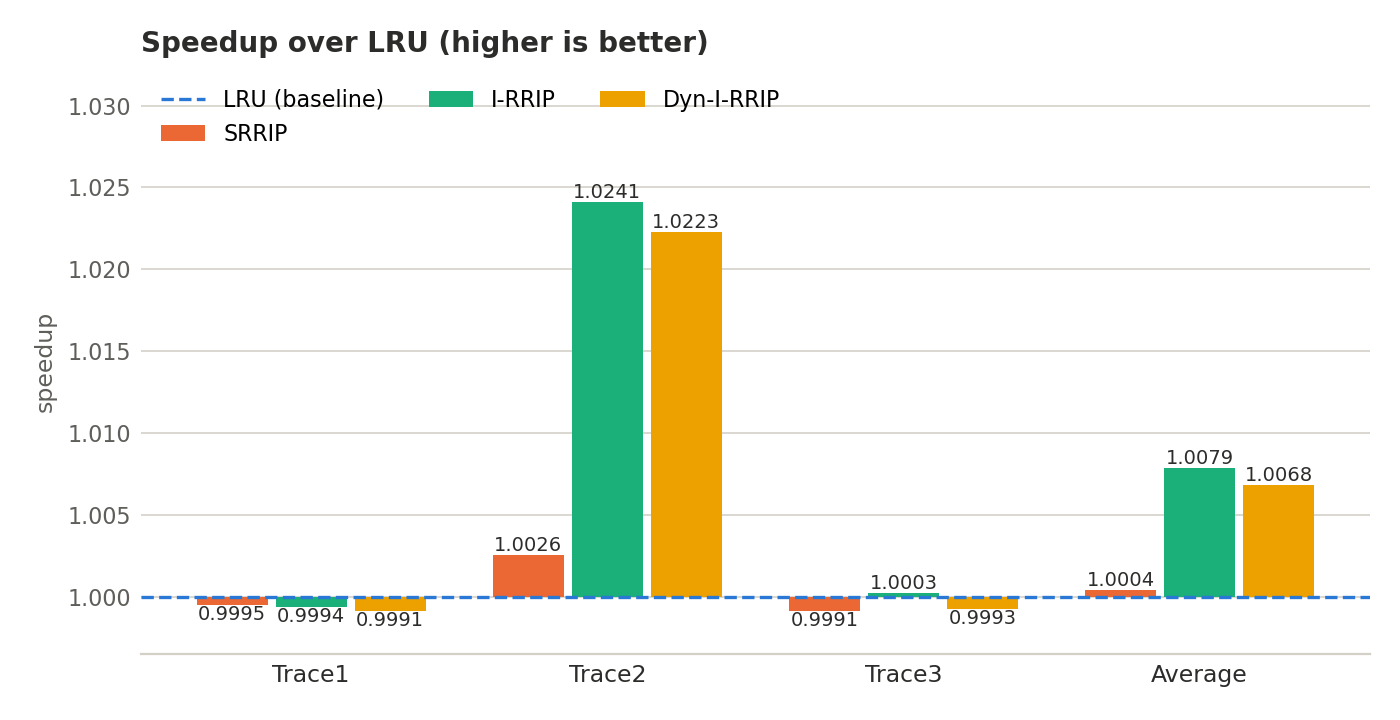
\includegraphics[width=0.49\linewidth]{task2b/plots/speedup.png}\hfill
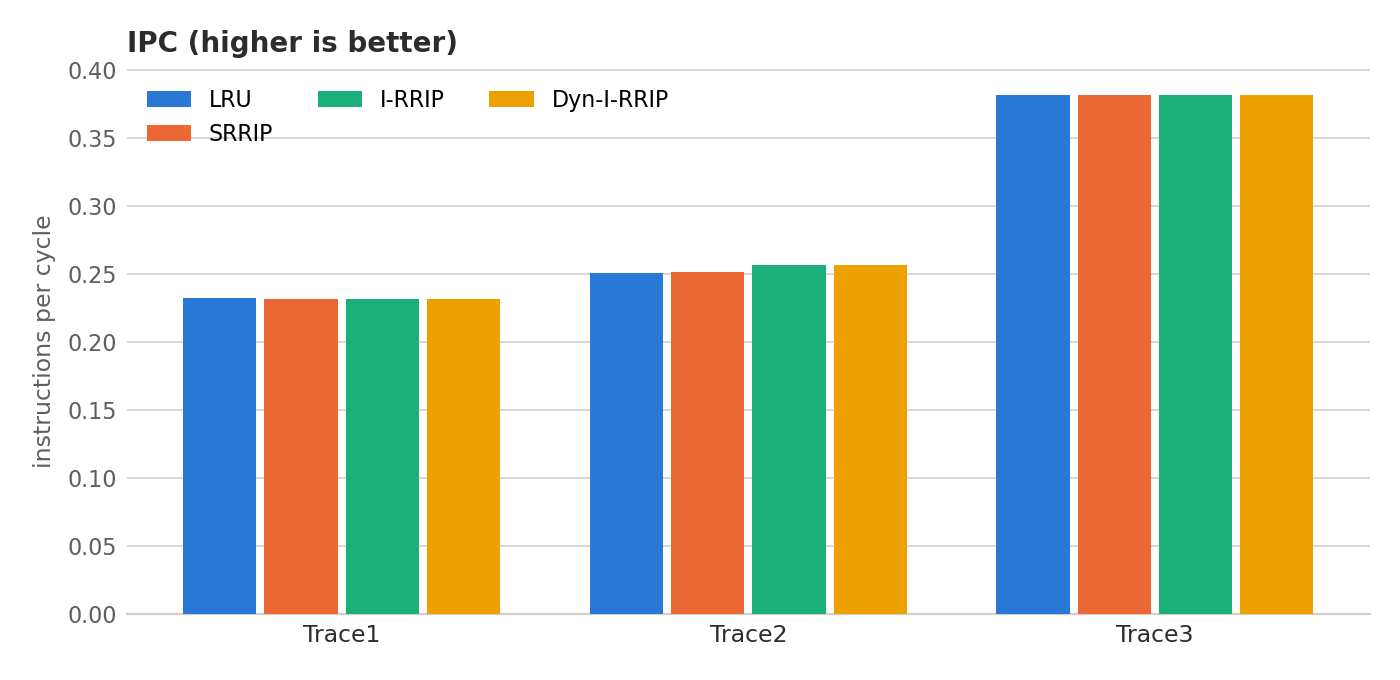
\includegraphics[width=0.49\linewidth]{task2b/plots/ipc.png}
\caption{Task 2B: speedup over LRU (dashed line: LRU = 1.0) and IPC per trace.}
\label{fig:t2b-speedup}
\end{figure}

\begin{figure}[H]
\centering
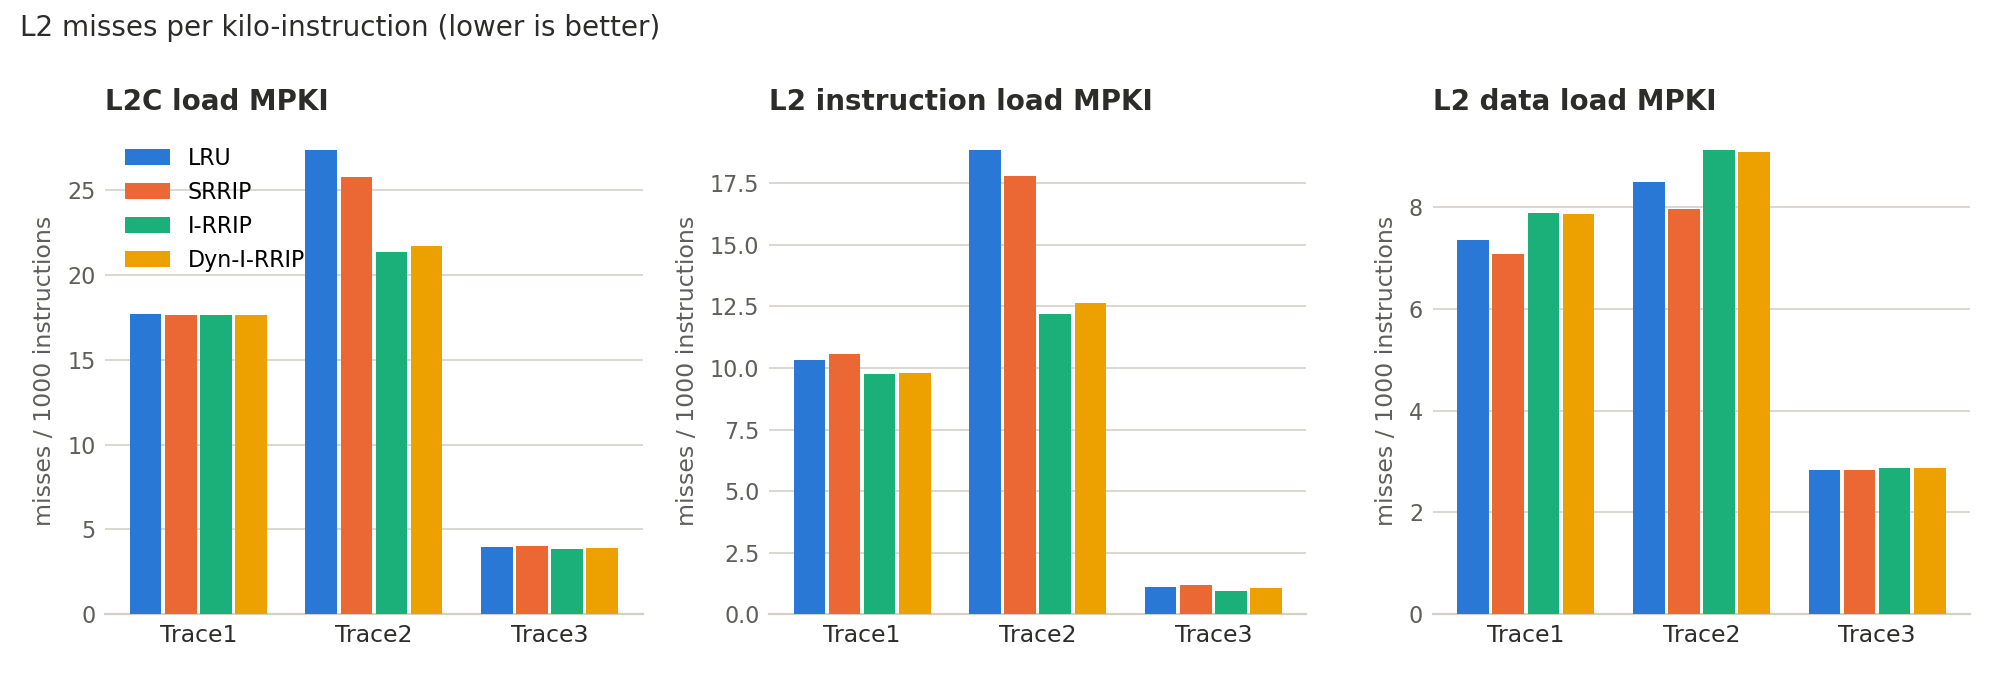
\includegraphics[width=0.9\linewidth]{task2b/plots/mpki.png}
\caption{Task 2B: L2 misses per 1000 instructions: all loads, instruction loads, data loads.}
\label{fig:t2b-mpki}
\end{figure}

\paragraph{Observations.}
\begin{itemize}
  \item \textbf{Dyn-I-RRIP still meets the Task 2A goal.} L2 instruction misses
        fall on every trace compared with LRU: $-5.3\%$ (Trace1), $-33.0\%$
        (Trace2), $-5.4\%$ (Trace3).
  \item \textbf{Trace2 is where it pays off:} 20.6\% fewer L2 load misses and
        2.23\% faster than LRU. The leaders measure an average ratio of 0.60
        there, far above the threshold, so 94\% of follower accesses are served
        in I-RRIP mode.
  \item \textbf{Trace1 and Trace3 stay within 0.1\% of LRU}, as with I-RRIP.
        Code and data effects cancel on these traces, so there is little to win
        or lose.
  \item \textbf{Against static I-RRIP} the dynamic policy is 0.10\% slower on
        average (0.18\% on Trace2); Section~\ref{sec:t2b-vs-static} explains why.
\end{itemize}

\subsection{Sensitivity study}
We varied the decision threshold over five values around the suggested 0.25
(32 leaders), and then the number of leader sets (16 / 32 / 64, threshold
0.25). Everything else was unchanged.

\begin{table}[H]
\centering
\small
\setlength{\tabcolsep}{4pt}
\begin{tabular}{rlrrrrrrr}
\toprule
Thresh. & Trace & IPC & Speedup & L2C load & L2 instr. & L2 data & \% in I-RRIP & Switches\\
        &       &     &         & MPKI     & MPKI      & MPKI    & mode         & \\
\midrule
0.10 & Trace1 & 0.2322 & 0.9995 & 17.649 &  9.789 & 7.860 & 100.0 & 0\\
     & Trace2 & 0.2571 & 1.0235 & 21.453 & 12.349 & 9.104 & 100.0 & 0\\
     & Trace3 & 0.3821 & 1.0002 &  3.831 &  0.966 & 2.865 & 100.0 & 0\\
     & Average &       & 1.0077 & & & & & \\
\midrule
0.20 & Trace1 & 0.2321 & 0.9991 & 17.651 &  9.788 & 7.864 & 100.0 & 0\\
     & Trace2 & 0.2568 & 1.0223 & 21.724 & 12.629 & 9.095 &  95.8 & 2\\
     & Trace3 & 0.3819 & 0.9996 &  3.914 &  1.052 & 2.863 &  71.9 & 1\\
     & Average &       & 1.0069 & & & & & \\
\midrule
0.25 & Trace1 & 0.2321 & 0.9991 & 17.651 &  9.788 & 7.864 & 100.0 & 0\\
     & Trace2 & 0.2568 & 1.0223 & 21.724 & 12.631 & 9.093 &  93.7 & 2\\
     & Trace3 & 0.3818 & 0.9993 &  3.931 &  1.064 & 2.868 &  57.5 & 1\\
     & Average &       & 1.0068 & & & & & \\
\midrule
0.30 & Trace1 & 0.2322 & 0.9992 & 17.680 &  9.810 & 7.870 & 100.0 & 0\\
     & Trace2 & 0.2567 & 1.0222 & 21.731 & 12.637 & 9.094 &  93.7 & 2\\
     & Trace3 & 0.3817 & 0.9991 &  3.998 &  1.121 & 2.878 &  42.3 & 1\\
     & Average &       & 1.0068 & & & & & \\
\midrule
0.40 & Trace1 & 0.2322 & 0.9993 & 17.604 &  9.841 & 7.762 &  88.4 & 4\\
     & Trace2 & 0.2565 & 1.0214 & 21.892 & 12.820 & 9.072 &  91.5 & 2\\
     & Trace3 & 0.3817 & 0.9991 &  3.998 &  1.119 & 2.878 &  42.5 & 1\\
     & Average &       & 1.0065 & & & & & \\
\bottomrule
\end{tabular}
\caption{Threshold sensitivity (32 leader sets). ``\% in I-RRIP mode'' = share
of follower accesses served in I-RRIP mode; ``Switches'' = mode changes after
warmup.}
\label{tab:t2b-threshold}
\end{table}

\begin{figure}[H]
\centering
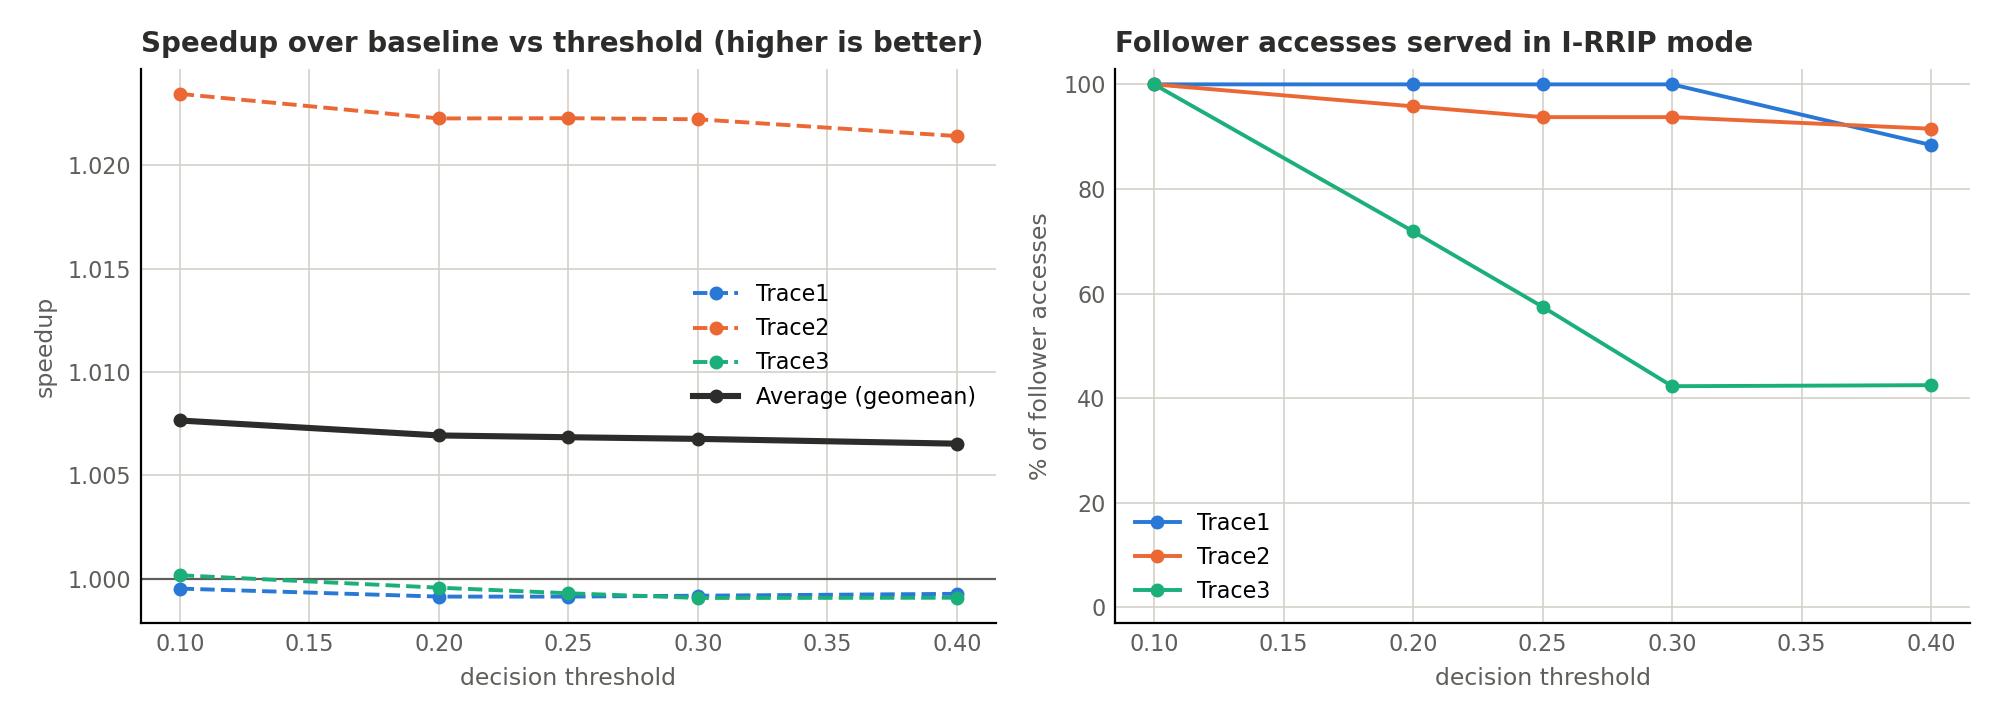
\includegraphics[width=0.95\linewidth]{task2b/plots/sensitivity.png}
\caption{Left: speedup vs.\ threshold. Right: share of time the followers spend
in I-RRIP mode.}
\label{fig:t2b-sensitivity}
\end{figure}

\begin{table}[H]
\centering
\small
\setlength{\tabcolsep}{4pt}
\begin{tabular}{rrrrrrr}
\toprule
Leader sets & \% of cache & Trace1 & Trace2 & Trace3 & Avg.\ speedup & Trace2 instr.\ MPKI\\
\midrule
16 & 1.6\% & 0.9994 & 1.0219 & 0.9997 & 1.0069 & 12.691\\
32 & 3.1\% & 0.9991 & 1.0223 & 0.9993 & 1.0068 & 12.631\\
64 & 6.3\% & 0.9994 & 1.0222 & 0.9991 & 1.0068 & 12.693\\
\bottomrule
\end{tabular}
\caption{Leader-set sensitivity (threshold 0.25). Speedups over LRU.}
\label{tab:t2b-leaders}
\end{table}

\paragraph{What the sensitivity study shows.}
\begin{itemize}
  \item \textbf{The result is flat.} Over a 4$\times$ range of thresholds the
        average speedup only moves between 1.0065 and 1.0077 (0.12\% spread);
        Trace2 stays between 1.0214 and 1.0235. A wrong threshold costs little.
  \item \textbf{Why it is flat:} the leaders measure an average ratio of about
        0.44 on Trace1 and 0.60 on Trace2, above every threshold we tried. Only
        Trace3 (average ratio 0.31) sits close to the thresholds, and its time
        in I-RRIP mode falls from 100\% to 42\% as the threshold rises
        (Figure~\ref{fig:t2b-sensitivity}, right). Since I-RRIP and SRRIP
        differ by only 0.1\% on Trace3, this barely shows in the speedup.
  \item \textbf{0.10 is the fastest (1.0077) but not really dynamic:} the ratio
        never drops that low, so the followers stay in I-RRIP mode 100\% of the
        time and the policy becomes static I-RRIP minus the 3\% of sets that the
        leaders keep in SRRIP.
  \item \textbf{0.40 starts to switch on Trace1} (4 switches, 88\% in I-RRIP).
        There data misses go down while code misses rise only slightly, but
        Trace2 is pushed out of I-RRIP mode more often and loses more, so the
        average is the lowest of the five.
  \item \textbf{We kept 0.25.} Among thresholds where switching actually
        happens, 0.20, 0.25 and 0.30 are equal within 0.02\%. 0.25 sits in the
        middle of that flat region, so it is the least sensitive choice, and it
        still lets the policy leave I-RRIP mode in a phase where code becomes a
        small part of the L2 traffic.
\end{itemize}

\subsection{Design choices}

\paragraph{Number of leader sets: 32.}
\begin{itemize}
  \item Too few leaders means a noisy sample: with 1024 accesses per window
        spread over only a few sets, a short burst in one set can decide the
        mode for the whole cache. More leaders also give more decisions per run
        (Trace2: 25 decisions with 16 leaders, 46 with 32, 97 with 64), so the
        policy reacts faster to a new phase.
  \item Too many leaders costs performance, because leader sets always run SRRIP
        and never get the I-RRIP benefit. With 64 leaders, 6.3\% of the cache is
        permanently in SRRIP mode.
  \item Measured: 16, 32 and 64 leaders give average speedups of 1.0069, 1.0068
        and 1.0068 (Table~\ref{tab:t2b-leaders}), the same within 0.01\%. With
        equal performance we chose the middle value: 32 leaders (3.1\% of sets)
        is the size commonly used for set dueling in a 1024-set cache (as in
        DIP/DRRIP), gives a sample twice as large as 16 for a less noisy
        decision, and loses half as many sets to SRRIP as 64.
\end{itemize}

\paragraph{Decision logic.}
\begin{itemize}
  \item \textbf{Leaders run SRRIP, not I-RRIP.} The policy asks ``how much does
        code matter if we don't protect it?''. Leaders running I-RRIP would hide
        code misses, the ratio would drop, and the policy would switch
        protection off exactly because protection was working.
  \item \textbf{Misses count twice in the ratio} (once as an access, once as a
        miss). A workload whose code mostly hits in the L2 has a lower ratio
        than one whose code keeps missing, which is what we want: protection
        only helps when code is being lost.
  \item \textbf{Window of 1024 leader accesses + halving.} A fixed window gives
        regular decisions; halving keeps a memory of about the last two windows.
        During the 25M measured instructions this gave 26 / 46 / 6 decisions and
        only 0 / 2 / 1 switches on Trace1 / 2 / 3: the policy follows real phase
        changes but does not thrash.
  \item \textbf{Threshold 0.25} from the assignment hint, kept after the
        sensitivity study.
\end{itemize}

\subsection{Why Dynamic I-RRIP does not beat static I-RRIP on these traces}
\label{sec:t2b-vs-static}
This is expected and does not mean the dynamic policy is wrong. Two things cost
it a little:
\begin{itemize}
  \item \textbf{The leaders never use I-RRIP.} 3.1\% of the cache always runs
        SRRIP, so on a trace where I-RRIP is always the right choice (Trace1,
        Trace2) the dynamic policy gives up the I-RRIP gain in those sets. This
        is the fixed price of set dueling: Trace2 runs in I-RRIP mode for 94\%
        of follower accesses and still loses 0.18\%.
  \item \textbf{Switching only helps if the other mode is better.} When Trace3
        drops into SRRIP mode (43\% of the time) it falls from I-RRIP's 1.0003 to
        0.9993, because on Trace3 SRRIP is slightly worse than I-RRIP (Task 2A:
        0.9991 vs.\ 1.0003).
\end{itemize}
The deeper reason is that on these three traces static I-RRIP never really
loses: its worst result is $-0.06\%$ (Trace1). A dynamic policy pays the small
set-dueling cost to protect against a case that does not occur here. It would
win on a workload with a long data-heavy phase where code fits in the L1I, where
static I-RRIP would raise data misses for nothing (on Trace1 static I-RRIP
already raises data misses by 7\%). The ratio also measures how much code the L2
sees rather than directly comparing the misses of the two policies. A natural
next step would be a second group of leaders running I-RRIP and comparing the
misses of both groups; we kept the single-group design from the hint because it
is cheaper and its loss here is only 0.10\%.

\subsection{Storage overhead}

\begin{table}[H]
\centering
\begin{tabular}{p{0.45\linewidth}p{0.45\linewidth}}
\toprule
Stored state & Size (L2: 1024 sets $\times$ 8 ways = 8192 lines)\\
\midrule
RRPV, 2 bits per line (same as SRRIP / I-RRIP) & $8192 \times 2$ bits = 2\,KB\\
Instruction bit, 1 bit per line (same as I-RRIP) & $8192 \times 1$ bit = 1\,KB\\
Leader-set flag & 0 bits: computed from the set index (two 5-bit fields compared)\\
4 counters: instruction/total accesses and misses & $4 \times 12$ bits = 48 bits (halving keeps each value $\le 2047$)\\
Window counter (0--1024) & 11 bits\\
Follower mode bit (I-RRIP / SRRIP) & 1 bit\\
\midrule
\textbf{Total} & \textbf{3\,KB + 60 bits} (under 8 bytes more than I-RRIP; about 0.6\% of the 512\,KB cache)\\
\bottomrule
\end{tabular}
\caption{Storage needed by Dynamic I-RRIP.}
\label{tab:t2b-storage}
\end{table}

%======================================================================
\section{Task 3: SPP with Prefetch-Aware Dynamic I-RRIP}

Policy file: \texttt{replacement/dyn\_irrip.l2c\_repl} (SPP at the L1D,
\texttt{prefetcher/spp.l1d\_pref}, unchanged from Task 1B).

\subsection{Design}
SPP issues its prefetches with \texttt{FILL\_L1}. A prefetch that misses in the
L2 is fetched from the LLC/DRAM and filled into \emph{both} the L2 and the L1D.
The L2 replacement policy sees these requests with \texttt{type == PREFETCH}.
Task 3 adds one rule set for them to Dynamic I-RRIP. It is applied in every set
(leader and follower) and in both follower modes, before any other rule:

\begin{table}[H]
\centering
\small
\begin{tabular}{p{0.27\linewidth}p{0.3\linewidth}p{0.33\linewidth}}
\toprule
Event & Dynamic I-RRIP (Task 2B) & Prefetch-aware Dynamic I-RRIP\\
\midrule
Prefetch fill (miss in L2) & inserted like a data line (RRPV 2) & RRPV 3\\
Prefetch hit in L2 & promoted like a data hit (RRPV 0 or 1) & RRPV unchanged\\
Prefetch in a leader set & counted in the dueling ratio & not counted\\
Demand hit on a prefetched line & -- & promoted as usual (code 0 / data 1 or 0)\\
\bottomrule
\end{tabular}
\caption{Prefetch handling added to Dynamic I-RRIP.}
\label{tab:t3-rules}
\end{table}

The rules only use the request type that the cache already passes to
\texttt{update\_replacement\_state()}, so they need \textbf{no extra storage}:
the total stays at 3\,KB + 60 bits (Table~\ref{tab:t2b-storage}). Nothing
needs to remember that a line was prefetched; once a demand load hits it, it is
treated like any other line.

\subsection{Rationale for handling prefetch packets}

\paragraph{The L2 copy of a prefetched line is rarely used.}
The L1D copy serves the program; the L2 copy is only read if the line is
evicted from the L1D and then requested again while still in the L2. With SPP
and LRU at the L2, only 7.4\%, 15.1\% and 5.0\% of the lines that SPP filled
into the L2 were ever hit by a demand load (Table~\ref{tab:t3-pf}). Under
Dynamic I-RRIP such a line would be inserted at RRPV 2 like demand data and,
on a hit by a later prefetch, promoted like reused data. It would then occupy
an L2 way for a long time and push out instruction lines, which is exactly
what I-RRIP tries to prevent.

\paragraph{Insertion at RRPV 3.}
A prefetched line is a data line already at the maximum RRPV, so it is the
first victim of the data-first eviction rule in I-RRIP mode and of the
first-at-RRPV-3 rule in SRRIP mode. It is evicted before any instruction line
and before demand data that has not aged yet. If the program does read it from
the L2, the demand hit promotes it normally, so a useful prefetch is not lost.
The measured cost is small: the share of L2 prefetch fills used by a demand
load falls to 1.0\%, 3.2\% and 1.2\%, i.e.\ about 1300, 250 and 350 fewer L2
hits per 25M instructions (at most 0.05 MPKI).

\paragraph{No promotion on a prefetch hit.}
A prefetch that hits in the L2 means the L1D is about to receive a copy of the
line. That is not a use by the program, and after it the program reads the
line from the L1D, not from the L2. Promoting the L2 copy would protect it
exactly while it is least needed. Only demand hits (and, as in Task 2A, not
writebacks) count as reuse.

\paragraph{Prefetches are not counted by the leader sets.}
The dueling ratio measures how much of the program's L2 demand traffic is
instruction traffic. Every SPP prefetch is a data request
(\texttt{L2C INSTRUCTION PREFETCH MPKI} is 0), and most of them miss in the
L2, so counting them would add to the denominator twice and lower the ratio
just because the prefetcher is active. On Trace3, whose ratio (0.35) is the
closest to the 0.25 threshold, the 9910 prefetches (9590 misses) would add
about 9\% to the denominator (131k L2 load accesses + 91k misses) and pull the
ratio towards the threshold. With prefetches excluded, the leaders measure
nearly the same ratio as Dynamic I-RRIP without a prefetcher
(Table~\ref{tab:t3-duel}), so the mode decision keeps reflecting code demand.
Writebacks are excluded for the same reason.

\subsection{Experimental setup}
Four configurations are compared on each trace:
\begin{itemize}
  \item \textbf{No prefetching (LRU)}: the Task 1B baseline; all speedups are
        relative to this run.
  \item \textbf{SPP (LRU)}: SPP at the L1D, LRU at the L2 (Task 1B).
  \item \textbf{Dyn-I-RRIP}: no prefetcher, Dynamic I-RRIP at the L2 (Task 2B).
  \item \textbf{SPP + PF-aware Dyn-I-RRIP}: SPP at the L1D, prefetch-aware
        Dynamic I-RRIP at the L2 (Task 3; threshold 0.25, 32 leaders, window
        1024).
\end{itemize}
Every other cache uses LRU and no other prefetcher is active. Tables and plots
are produced by \texttt{scripts/task3\_metrics.py}
(\texttt{results/task3/task3\_metrics.csv}, \texttt{task3\_table.md},
\texttt{plots/}).

The four configurations come from runs made at different times and on
different machines. Two equivalent no-prefetching LRU runs (Task 1B baseline
and Task 2B LRU) differ by up to 0.06\% in IPC and by up to 0.54 L2 instruction
MPKI (Trace2), so differences of that size are within noise. For the same
reason Dyn-I-RRIP's speedups here (vs.\ the Task 1B baseline) differ slightly
from Table~\ref{tab:t2b-results} (vs.\ the Task 2B LRU run).

\subsection{Results}

\begin{table}[H]
\centering
\small
\setlength{\tabcolsep}{4pt}
\begin{tabular}{l rrrr rrr}
\toprule
& \multicolumn{4}{c}{IPC} & \multicolumn{3}{c}{Speedup over no prefetching (LRU)}\\
\cmidrule(lr){2-5}\cmidrule(lr){6-8}
Trace & No PF & SPP & Dyn-I-RRIP & SPP + PF-aware & SPP & Dyn-I-RRIP & SPP + PF-aware\\
\midrule
Trace1 & 0.2322 & \textbf{0.2332} & 0.2321 & 0.2327 & \textbf{1.0042} & 0.9997 & 1.0021\\
Trace2 & 0.2511 & 0.2513 & \textbf{0.2568} & 0.2552 & 1.0008 & \textbf{1.0224} & 1.0163\\
Trace3 & 0.3821 & 0.3829 & 0.3818 & \textbf{0.3830} & 1.0023 & 0.9993 & \textbf{1.0024}\\
\midrule
Average & 0.2885 & 0.2891 & 0.2902 & \textbf{0.2903} & 1.0024 & \textbf{1.0071} & 1.0069\\
\bottomrule
\end{tabular}
\caption{Task 3: IPC and speedup (Average: arithmetic mean for IPC, geometric
mean for speedup). Best value per row in bold.}
\label{tab:t3-ipc}
\end{table}

\begin{table}[H]
\centering
\small
\begin{tabular}{llrrrr}
\toprule
Trace & Configuration & L1D load & L2C load & L2 instr. & L2 data\\
      &               & MPKI     & MPKI     & MPKI      & MPKI\\
\midrule
Trace1 & No prefetching (LRU)      & 10.679 & 17.730 & 10.384 & 7.346\\
       & SPP (LRU)                 & 10.062 & 17.214 & 10.389 & 6.825\\
       & Dyn-I-RRIP                & 10.680 & 17.651 &  9.788 & 7.864\\
       & SPP + PF-aware Dyn-I-RRIP & 10.072 & 17.172 &  9.848 & 7.323\\
\midrule
Trace2 & No prefetching (LRU)      & 13.534 & 27.923 & 19.391 & 8.533\\
       & SPP (LRU)                 & 13.446 & 27.827 & 19.326 & 8.500\\
       & Dyn-I-RRIP                & 13.541 & 21.724 & 12.631 & 9.093\\
       & SPP + PF-aware Dyn-I-RRIP & 13.457 & 23.206 & 14.218 & 8.988\\
\midrule
Trace3 & No prefetching (LRU)      &  3.403 &  3.959 &  1.126 & 2.833\\
       & SPP (LRU)                 &  3.285 &  3.703 &  1.129 & 2.574\\
       & Dyn-I-RRIP                &  3.403 &  3.931 &  1.064 & 2.868\\
       & SPP + PF-aware Dyn-I-RRIP &  3.277 &  3.649 &  1.053 & 2.595\\
\midrule
Average & No prefetching (LRU)      & 9.205 & 16.538 & 10.300 & 6.237\\
        & SPP (LRU)                 & 8.931 & 16.248 & 10.281 & 5.967\\
        & Dyn-I-RRIP                & 9.208 & 14.436 &  7.827 & 6.608\\
        & SPP + PF-aware Dyn-I-RRIP & 8.935 & 14.675 &  8.373 & 6.302\\
\bottomrule
\end{tabular}
\caption{Task 3: load MPKI of the L1D, the L2C, and L2 instruction and data
loads.}
\label{tab:t3-mpki}
\end{table}

\begin{table}[H]
\centering
\small
\setlength{\tabcolsep}{4pt}
\begin{tabular}{ll rrrr rrr}
\toprule
& & \multicolumn{4}{c}{L1D} & \multicolumn{3}{c}{L2 copies of prefetched lines}\\
\cmidrule(lr){3-6}\cmidrule(lr){7-9}
Trace & Configuration & Accuracy & Coverage & PF issued & PF useful & Fills & Demand hits & \% used\\
\midrule
Trace1 & SPP (LRU)       & 60.72\% & 5.78\% & 28454 & 17278 & 20484 & 1513 &  7.39\\
       & SPP + PF-aware  & 60.94\% & 5.69\% & 27752 & 16913 & 21985 &  221 &  1.01\\
\midrule
Trace2 & SPP (LRU)       & 57.47\% & 0.65\% &  5211 &  2995 &  2279 &  345 & 15.14\\
       & SPP + PF-aware  & 56.67\% & 0.57\% &  5394 &  3057 &  2890 &   93 &  3.22\\
\midrule
Trace3 & SPP (LRU)       & 33.36\% & 3.48\% &  9496 &  3168 &  9112 &  455 &  4.99\\
       & SPP + PF-aware  & 33.73\% & 3.70\% &  9910 &  3343 &  9590 &  110 &  1.15\\
\midrule
Average & SPP (LRU)      & 50.52\% & 3.30\% & & & & & \\
        & SPP + PF-aware & 50.45\% & 3.32\% & & & & & \\
\bottomrule
\end{tabular}
\caption{Task 3: L1D prefetch accuracy and coverage, and what happens to the
L2 copies of prefetched lines (fills = prefetches that missed in the L2;
demand hits = those L2 lines later hit by a demand load). ``SPP + PF-aware'' =
SPP + prefetch-aware Dyn-I-RRIP.}
\label{tab:t3-pf}
\end{table}

\begin{table}[H]
\centering
\small
\begin{tabular}{l rr rr rr}
\toprule
& \multicolumn{2}{c}{Average ratio} & \multicolumn{2}{c}{\% in I-RRIP mode} & \multicolumn{2}{c}{Mode switches}\\
\cmidrule(lr){2-3}\cmidrule(lr){4-5}\cmidrule(lr){6-7}
Trace & Dyn & SPP + Dyn & Dyn & SPP + Dyn & Dyn & SPP + Dyn\\
\midrule
Trace1 & 0.439 & 0.445 & 100.0 & 100.0 & 0 & 0\\
Trace2 & 0.600 & 0.634 &  93.7 &  95.8 & 2 & 2\\
Trace3 & 0.308 & 0.350 &  57.5 &  63.8 & 1 & 1\\
\bottomrule
\end{tabular}
\caption{Set-dueling decision of Dynamic I-RRIP without a prefetcher (Dyn) and with SPP and the prefetch rules (SPP + Dyn). ``\% in I-RRIP mode'' = share of follower accesses served in I-RRIP mode.}
\label{tab:t3-duel}
\end{table}

\begin{figure}[H]
\centering
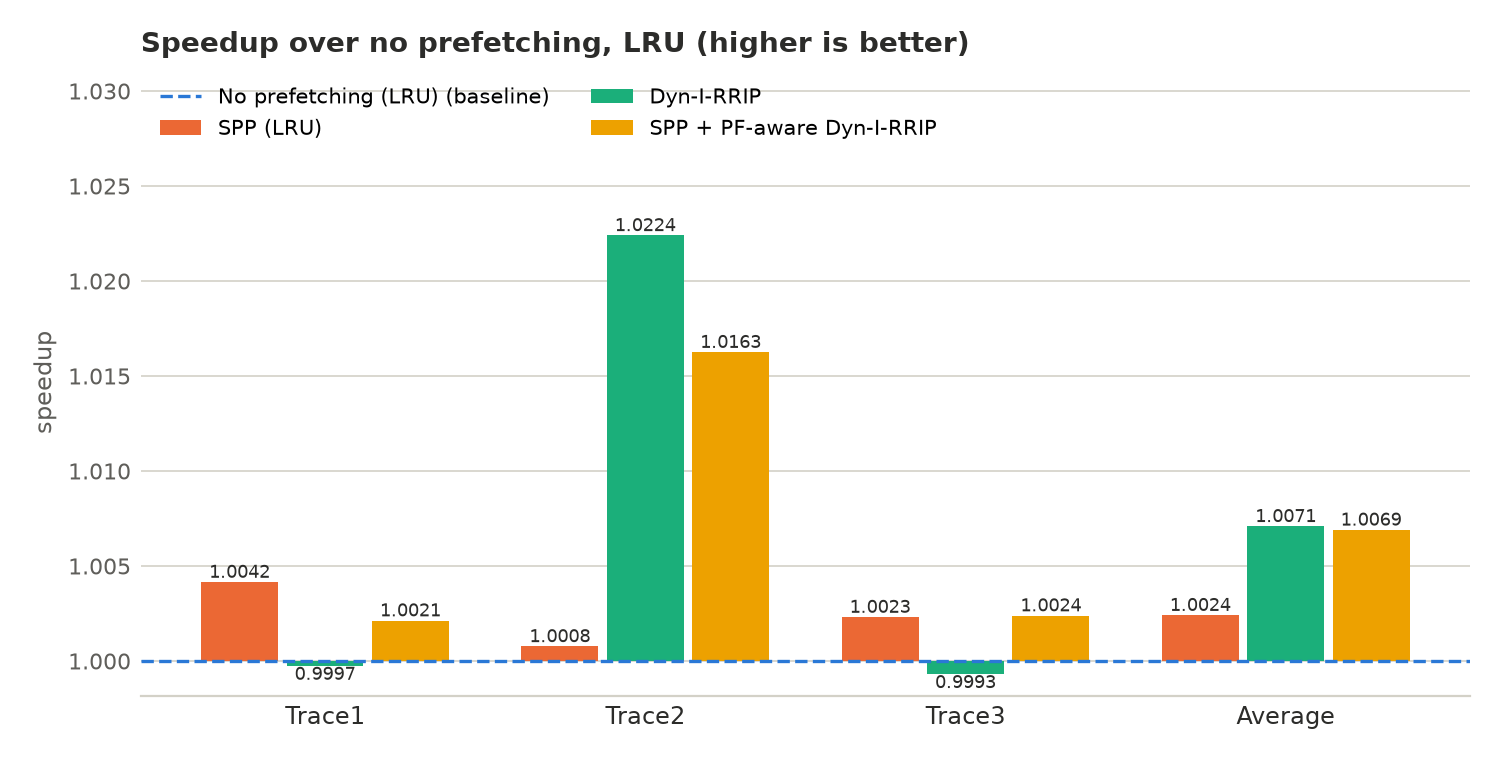
\includegraphics[width=0.49\linewidth]{task3/plots/speedup.png}\hfill
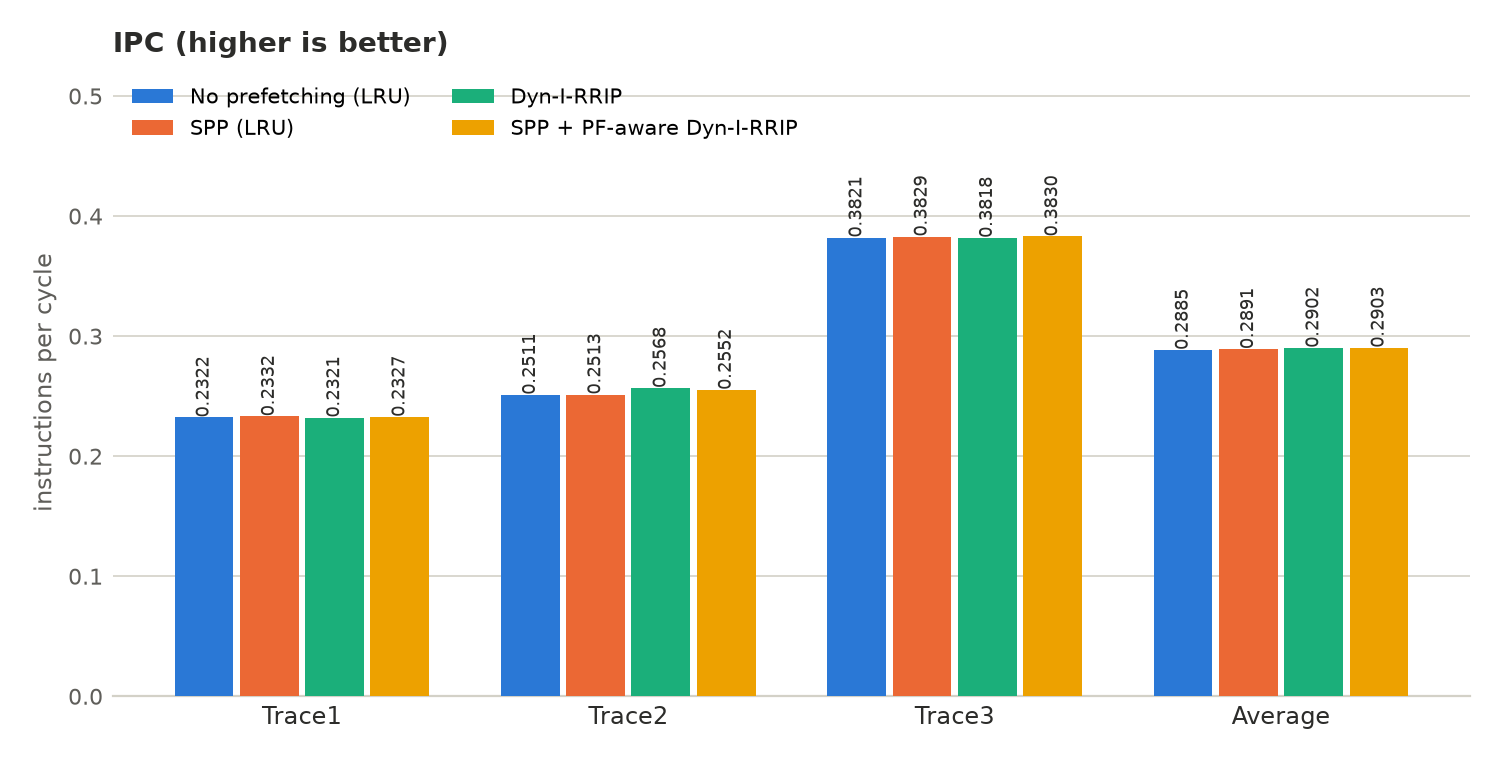
\includegraphics[width=0.49\linewidth]{task3/plots/ipc.png}
\caption{Task 3: speedup over no prefetching with LRU (dashed line) and IPC.}
\label{fig:t3-speedup}
\end{figure}

\begin{figure}[H]
\centering
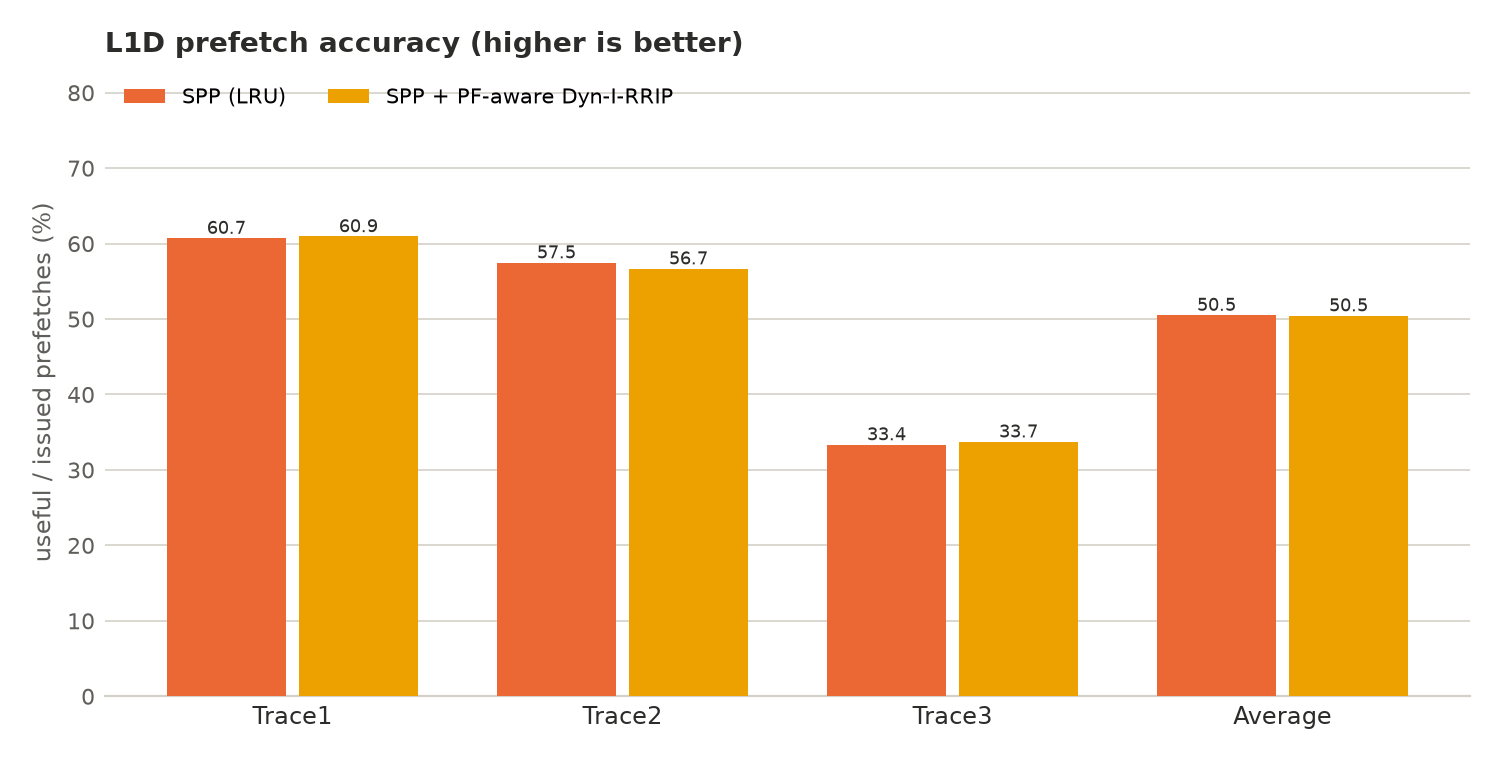
\includegraphics[width=0.49\linewidth]{task3/plots/accuracy.png}\hfill
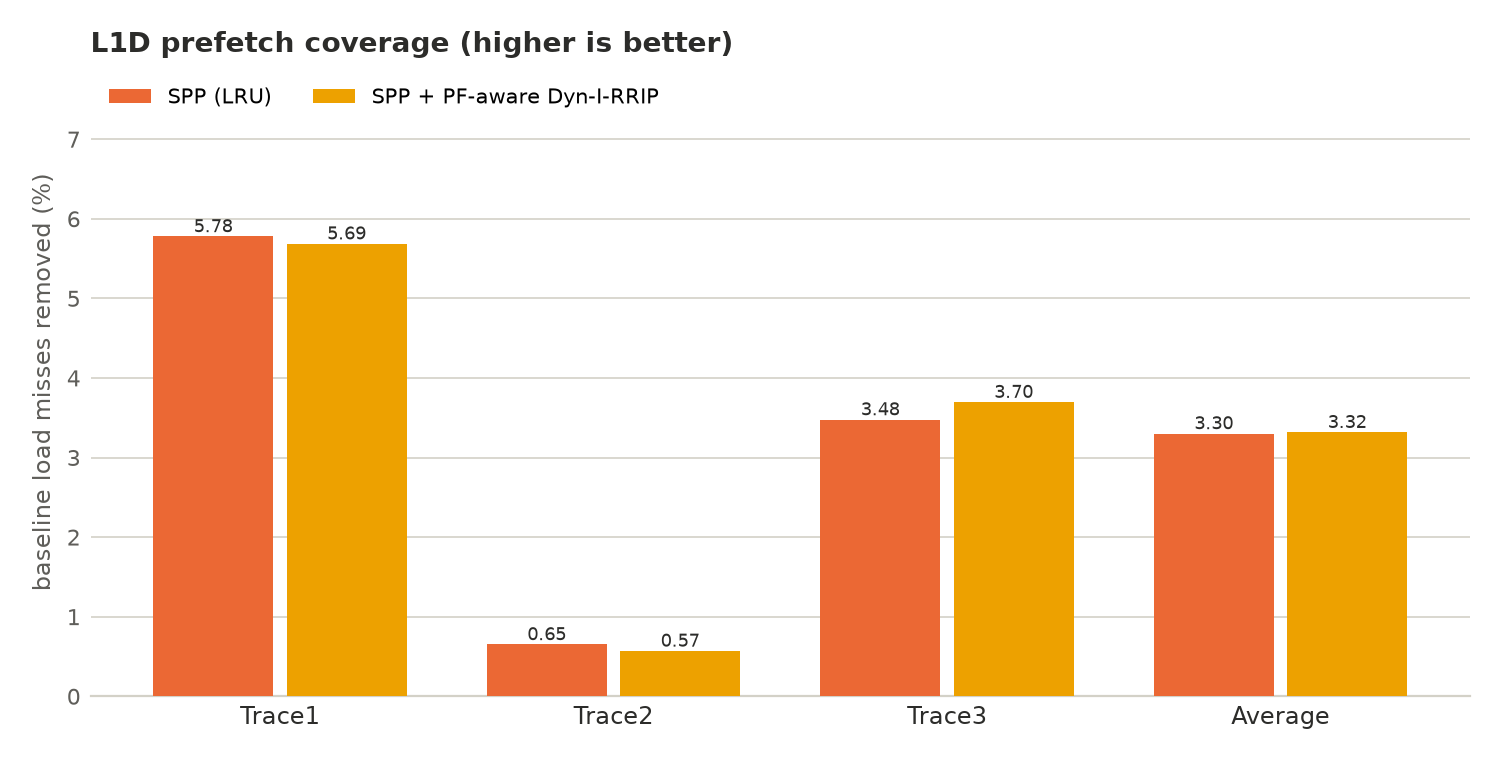
\includegraphics[width=0.49\linewidth]{task3/plots/coverage.png}
\caption{Task 3: L1D prefetch accuracy and coverage of SPP with LRU and with
prefetch-aware Dynamic I-RRIP at the L2.}
\label{fig:t3-pf}
\end{figure}

\begin{figure}[H]
\centering
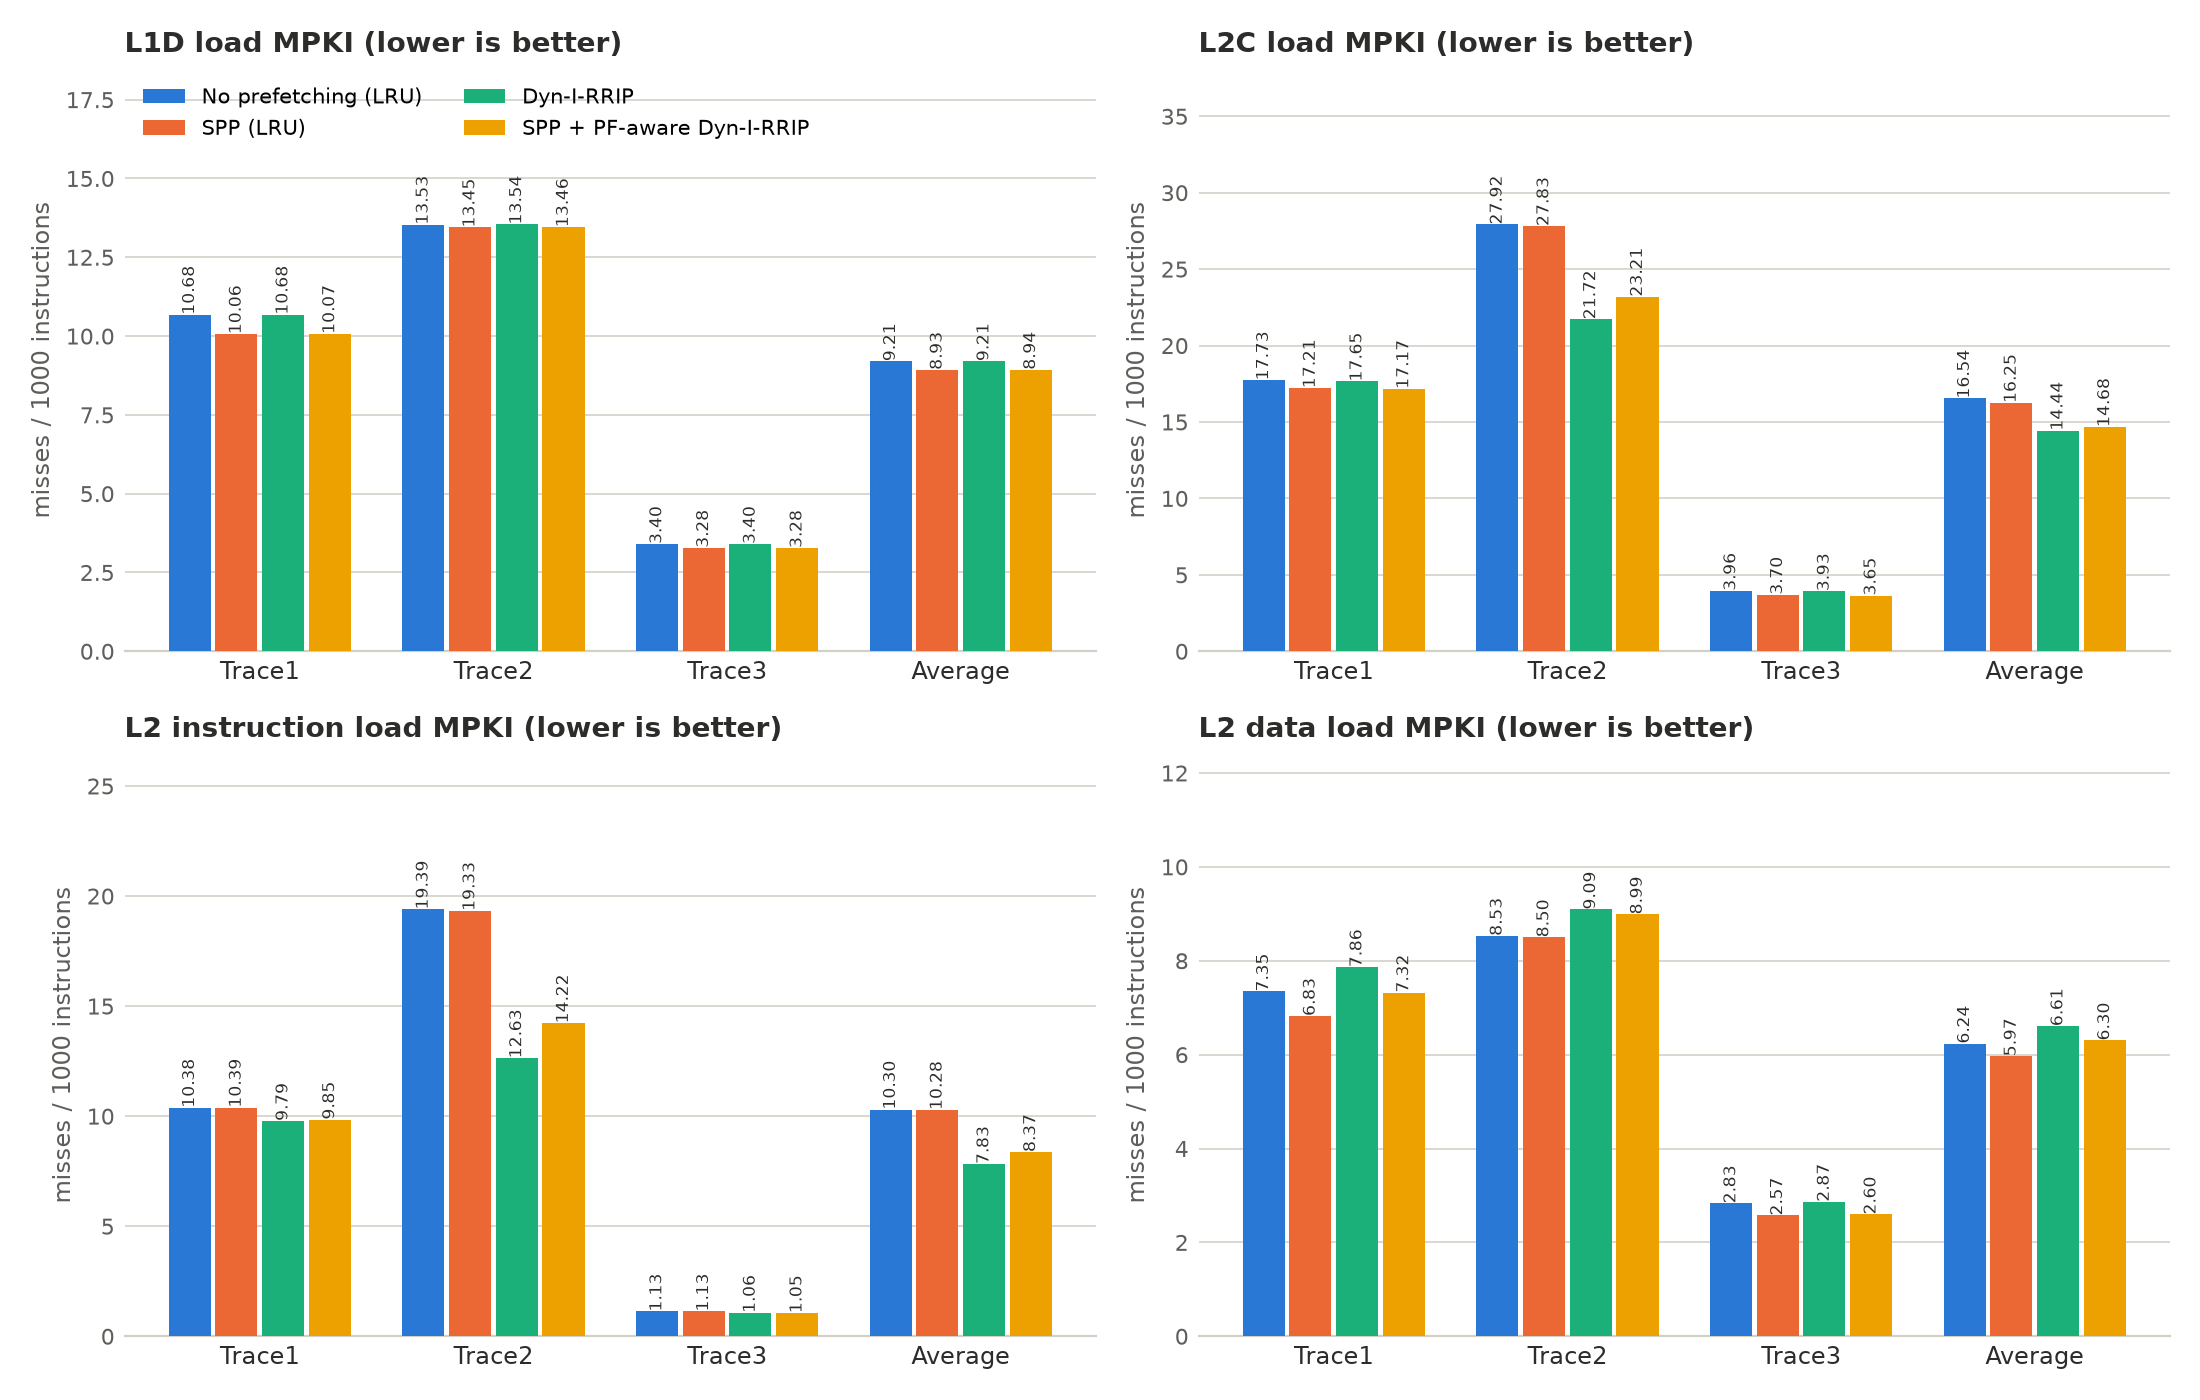
\includegraphics[width=\linewidth]{task3/plots/mpki.png}
\caption{Task 3: L1D, L2C, L2 instruction and L2 data load MPKI.}
\label{fig:t3-mpki}
\end{figure}

\subsection{Observations}
\begin{itemize}
  \item \textbf{The two mechanisms combine on the misses they target.} The
        combination keeps SPP's L1D benefit (L1D load MPKI 8.935 vs.\ 8.931 for
        SPP alone; same accuracy and coverage within 1\%) and most of Dynamic
        I-RRIP's L2 instruction benefit (average L2 instruction MPKI 8.373 vs.\
        10.281 for SPP with LRU). It also has the lowest L2C load MPKI on Trace1
        and Trace3.
  \item \textbf{SPP behaves the same under the new L2 policy.} L1D accuracy and
        coverage are unchanged within noise (Table~\ref{tab:t3-pf}), so inserting
        prefetched lines at RRPV 3 in the L2 does not hurt the prefetcher: what
        matters to it is the L1D copy.
  \item \textbf{The prefetch rules do what they are meant to.} The L2 copies of
        prefetched lines are evicted quickly (1--3\% are reused instead of
        5--15\%), and the dueling ratio and the time spent in I-RRIP mode stay at
        the level of Dynamic I-RRIP without a prefetcher
        (Table~\ref{tab:t3-duel}).
  \item \textbf{IPC.} The combination has the highest average IPC (0.2903 vs.\
        0.2902 for Dyn-I-RRIP and 0.2891 for SPP) and is the best configuration
        on Trace3 (1.0024). Its geometric-mean speedup (1.0069) is equal to
        Dynamic I-RRIP's (1.0071) within noise and well above SPP's (1.0024).
        It does \emph{not} beat both standalone mechanisms on every trace: on
        Trace1 it is between them (1.0021 vs.\ SPP's 1.0042), and on Trace2 it is
        0.6\% behind Dynamic I-RRIP (1.0163 vs.\ 1.0224).
  \item \textbf{Trace2.} The combination has 1.6 more L2 instruction MPKI than
        Dynamic I-RRIP alone (14.22 vs.\ 12.63). Up to about 0.5 MPKI of that is
        run-to-run difference between the two setups (see the setup above); the
        rest means prefetches still cost some code lines even at RRPV 3. A likely
        cause is the victim search: when a prefetch fill finds no line at RRPV 3,
        every line in the set is aged, including instruction lines, which brings
        them closer to eviction.
\end{itemize}

\end{document}
